\documentclass[a4paper, openany, 12pt]{extarticle}

%% подключаем преамбулу: в ней содержится подключение всех необходимых пакетов
%% Работа с русским языком
\usepackage{cmap}			 % поиск в PDF
\usepackage{mathtext} 		 % русские буквы в формулах
\usepackage[T2A]{fontenc}	 % кодировка
\usepackage[utf8]{inputenc}	 % кодировка исходного текста
\usepackage[russian]{babel}	 % локализация и переносы

%% Пакеты для работы с математикой
\usepackage{amsmath,amsfonts,amssymb,amsthm,mathtools}
\usepackage{icomma}

%% Нумерация формул (опционально)
%\mathtoolsset{showonlyrefs=true} % показывать номера только у тех формул, на которые есть \eqref{} в тексте.
%\usepackage{leqno}               % нумерация формул слева

%% Шрифты
\usepackage{euscript}	 % шрифт "Евклид"
\usepackage{mathrsfs}    % красивый мат. шрифт

%% Некоторые полезные макросы для дебага (в случае недоверия авторам шаблона)
\makeatletter
\newcommand\thefontsize{The current font size is: \f@size pt} % пример: \section{\thefontsize}
\makeatother

%% Настройка размеров шрифтов
\makeatletter
\setlength{\headheight}{28pt}
\setlength{\marginparwidth}{2cm}
%% TODO: мне не удалось разобраться, как грамотно подбирать второе число в
%% \@setfontsize\*, но ряд экспериментов показывает, что "10" выравнивает текст весьма прилично :)
\renewcommand\Huge{\@setfontsize\Huge{14pt}{10}}
\renewcommand\huge{\@setfontsize\huge{14pt}{10}}
\renewcommand\Large{\@setfontsize\Large{14pt}{10}}
\renewcommand\large{\@setfontsize\large{12pt}{10}}
\makeatother

%% Поля (геометрия страницы)
\usepackage[left=2.5cm,right=1cm,top=2cm,bottom=2cm,bindingoffset=0cm]{geometry}

%% Русские списки
\usepackage{enumitem}
\makeatletter
\AddEnumerateCounter{\asbuk}{\russian@alph}{щ}
\makeatother

%% Работа с картинками
\usepackage{caption}
\captionsetup{justification=centering} % центрирование подписей к картинкам
\usepackage{graphicx}                  % вставки рисунков
\graphicspath{{pics/}}     % папки с картинками
\setlength\fboxsep{3pt}                % отступ рамки \fbox{} от рисунка
\setlength\fboxrule{1pt}               % толщина линий рамки \fbox{}
\usepackage{wrapfig}                   % обтекание рисунков и таблиц текстом

%% Работа с таблицами
\usepackage[table]{xcolor}                  % цветная заливка строк в таблицах
\usepackage{array,tabularx,tabulary,booktabs} % дополнительная работа с таблицами
\usepackage{longtable}                        % длинные таблицы
\usepackage{multirow}                         % слияние строк в таблице

%% Красная строка
\setlength{\parindent}{3em}

%% Интервалы
\linespread{1.5}
\usepackage{multirow}

%% Верхний колонтитул
\usepackage{fancyhdr}
\pagestyle{fancy}

%% Перенос знаков в формулах (по Львовскому)
\newcommand*{\hm}[1]{#1\nobreak\discretionary{}{\hbox{$\mathsurround=0pt #1$}}{}}

%% Дополнительно
\usepackage{float}   % добавляет возможность работы с командой [H], которая улучшает расположение на странице
\usepackage{gensymb} % красивые градусы
\usepackage{caption} % пакет для подписей к рисункам, в частности, для работы caption*
\usepackage{listings} % пакет для листингов с кодом
\usepackage{placeins} % \FloatBarrier

% Hyperref (для ссылок внутри PDF)
\usepackage[unicode, pdftex]{hyperref}

% Отступ перед первым абзацем в каждом разделе
\usepackage{indentfirst}

% Красивые листинги с подсветкой
\usepackage[outputdir=build]{minted}
\setminted{baselinestretch=1}
\renewcommand{\listingscaption}{Листинг}


\usepackage[backend=biber, style=gost-numeric, % стиль цитирования и библиографии
language=auto, % получение языка из babel
autolang=other, % многоязычная библиография
]{biblatex}
\addbibresource{9__literature.bib}

\usepackage[order=letter,acronym,symbols,toc,hyperfirst,automake]{glossaries}
\usepackage[automake,acronym]{glossaries-extra}

\input{include/math.tex}

\newacronym{pic}{PIC}{Position Independent Code, позиционно независимый код}
\newacronym{got}{GOT}{Global Offset Table, таблица глобальных смещений}
\newacronym{plt}{PLT}{Procedure Linkage Table, таблица связывания процедур}
\newacronym{aslr}{ASLR}{Address Space Layout Randomization, рандомизация адресного пространства}
\newacronym{os}{ОС}{Операционная Система}
\newacronym{sw}{ПО}{Программное обеспечение}
\newacronym{vm}{ВМ}{Языковая Виртуальная Машина}
\newacronym{dfg}{ГПД}{Граф Потока Данных. Вершины графа моделируют исполнения инструкций (иногда называемые просто инструкциями), ребра - зависимости между инструкциями по значениям. С каждым ребром ассоциируются значение и локация, по которой данное значение располагается (также называемые значением и локацией ребра).}

\newglossaryentry{module}
{
    name={Модуль},
    description={Библиотека или приложение}
}

\newglossaryentry{unit-testing}{
    name={Юнит тестирование (unit testing)},
    description={Тестирование минимального фрагмента кода (функции или метода) в изоляции от других компонентов. Поведение внешних зависимостей имитируется с помощью объектов-подражателей (mock objects)}
}

\newglossaryentry{module-testing}{
    name={Модульное тестирование (module testing)},
    description={Тестирование группы связанных компонентов, образующих законченный модуль системы. Проверяет корректность взаимодействия внутри модуля и его интерфейсов}
}

\newglossaryentry{end-to-end-testing}{
    name={Сквозное тестирование (end to end testing)},
    description={Тестирование полного бизнес-сценария в условиях, максимально приближенных к реальным. Проверяет работу всех компонентов системы вместе, включая внешние зависимости}
}

\newglossaryentry{sink}
{
    name={Псевдо-инструкция},
    description={Вершина ГПД, не отвечающая реальной инструкции. Используется для отображения различных зависимостей на графе}
}

\newglossaryentry{addr_edge}
{
    name={Адресное ребро},
    description={Ребро ГПД, значение которого используется в качестве адреса}
}

\newglossaryentry{src_addr_edge}{
    name={Исходное адресное ребро},
    description={Ребро, на котором заканчивается построение обратного пути из адресного ребра на ГПД в алгоритме поиска адресов}
}

\newglossaryentry{trace}{
    name={Трасса исполнения},
    description={Набор упорядоченных записей о событиях, происходивших во время трассировочного запуска приложения}
}

\newglossaryentry{dfg_math}{
    name={$G = (V, E)$},
    description={ГПД, где: $\mathbf{V}$ - множество вершин графа, $\mathbf{E}$ - множество ребер графа},
    type=symbols
}

\newglossaryentry{edges_subsets}{
    name={$\mathbf{2^E}$},
    description={Множество всех подмножеств ребер ГПД},
    type=symbols
}

\makeglossaries


\begin{document}
    %% титульник
    \begin{center}
    %% *название института*
    \large\textbf{Министерство образования и науки Российской Федерации \\
    Московский физико-технический институт (государственный
    университет)} \\
    \vspace{1cm}

    %% *факультет/физтех-школа*
    Физтех-школа радиотехники и компьютерных технологий \\

    %% *название базовой кафедры и лаборатории*
    %% в случае ненадобности можно удалить
    Кафедра микропроцессорных технологий в интеллектуальных системах управления \\

    \vspace{3em}

    Выпускная квалификационная работа магистра
\end{center}

\begin{center}
    \vspace{\fill}
    %% *название вашей работы*
    \LARGE{Изменение трасс исполнения для модификации записанных образов памяти}

    \vspace{\fill}
\end{center}


\begin{flushright}
    \textbf{Автор:} \\
    Студент 407 группы \\
    Матренин Василий Николаевич \\
    \vspace{2em}
    \textbf{Научный руководитель:} \\
    Петушков Игорь Вячеславович \\
    \vspace{2em}
    \textbf{Научный консультант:} \\
    Матвеев Сергей Владимирович \\
\end{flushright}

\vspace{7em}

\begin{center}
    %% *лого*
    
\includegraphics[width=100 pt]{pics/MIPT_logo.jpg}\\
    Москва \the\year{}
\end{center}

%% выключаем отображение номера для этой страницы (титульник)
\thispagestyle{empty}

\newpage
\setcounter{page}{2}
\fancyfoot[c]{\thepage}
%% *надпись над верхним колонтитулом*
%% в случае ненадобности можно удалить
\fancyhead[L]{Изменение трасс исполнения для модификации записанных образов памяти}
\fancyhead[R]{}


    %% аннотация
    Трасса исполнения (далее -- трасса) представляет собой упорядоченный набор записей о событиях, происходивших в ходе трассировочного запуска приложения \cite{pinplay,whole_execution_traces}. Подобные трассы широко применяются в индустрии для решения различных задач, таких как исследование поведения приложений, анализ производительности платформ, отладка, сбор профилей исполнения для компиляторов \cite{pinplay,autofdo,lisitsyn_disser}. В рамках данной работы рассмотрены трассы для RISC-архитектуры.

Целевые сценарии исполнения, записанные в виде трасс, могут применяться для анализа поведения разрабатываемых платформ. При этом настройки системы памяти новой платформы (далее -- новая конфигурация или новые настройки) могут отличаться от настроек платформы, на которой были записаны трассы. Возникает необходимость адаптации трасс под новую конфигурацию системы памяти.

Целью данной работы является разработка решения, позволяющего изменять трассы исполнения для модификации записанных в них образов памяти приложений в соответствии с ограничениями новой конфигурации системы памяти.

Представленное решение осуществляет перенос областей образа памяти в соответствии с новыми ограничениями посредством поиска и модификации адресов и смещений в трассе. Для генерации необходимых модификаций анализируется граф потока данных трассы. Рассмотрены алгоритмы генерации карты перемещений областей памяти, сбора графа потока данных из трассы исполнения, поиска локаций адресов и смещений в трассе с помощью обходов графа, обработки граничных случаев с помощью симуляционного прохода по модифицированной трассе. Описанный подход позволяет обеспечить консистентность потоков управления и данных в результирующих трассах, а также снизить влияние модификаций на репрезентативность этих трасс. Представленные алгоритмы могут быть использованы для других задач, связанных с модификацией адресов и смещений в трассах исполнения.

Временная и пространственная сложность обработки трассы линейна по числу инструкций и связей по данным между ними. Предложена метрика для предварительной оценки влияния производимых модификаций на репрезентативность трасс. Рассмотрены другие метрики для количественной оценки свойств реализации. Представлены результаты экспериментальных запусков разработанного средства, результаты валидации выходных трасс и значения собираемых метрик на наборе целевых трасс заказчика для одной из рассматриваемых конфигураций: с увеличенным размером страниц и расширенными областями, зарезервированными под данные ядра ОС. Описаны возможности для дальнейшего улучшения разработанного средства и новые направления его применения.

Предложенное решение успешно применяется для анализа поведения разрабатываемой системы на целевых сценариях исполнения и конфигурациях системы памяти.

\newpage


    %% содержание
    \tableofcontents{}
    \newpage
    \printglossary[type=\acronymtype]
    \printglossary[type=symbols, title={Математические обозначения}]
    \printglossary[type=main]
    \newpage

    \section{Введение}

\subsection{Трассы исполнения} \label{sec:execution_traces}

\gls{trace} представляет собой упорядоченный набор записей о событиях: исполнениях инструкций, операциях с памятью, системных вызовах, сигналах и т. д., происходивших во время трассировочного запуска приложения.

Трассы исполнения применяются в индустрии для различных задач, таких как: микроархитектурный и макро анализ приложений, сбор профилей исполнения, отладка \cite{trace_checkpoint_for_dvfs,plc_behav_model_from_traces,atlantis_paper,pinplay,lisitsyn_disser}. В рамках данной работы рассмотрены трассы для RISC-архитектуры.

Трасса может содержать записи для нескольких потоков исполнения, однако для простоты в дальнейшем будем рассматривать только трассы исполнения с одним потоком. Описанное в данной работе решение нетрудно обобщается на трассы с произвольным числом потоков.

Будем называть \glsdisp{app_instr}{инструкцией приложения (статической инструкцией)} статическую машинную инструкцию, расположенную в памяти трассируемой программы. Записи трассы исполнения, отвечающие одному выполнению инструкции приложения назовем \glsdisp{trace_instr}{инструкцией трассы (динамической инструкцией)}. Далее, если не оговорено иное, под инструкцией понимается именно динамическая инструкция.

Рассматриваемые трассы исполнения содержат следующие основные виды записей:

\begin{itemize}
    \item Начальное регистровое состояние

    Содержит значения регистров общего назначения, векторных регистров и условных флагов в момент начала трассировки. Также такие записи используются для отображения состояния машины при переключениях контекста исполнения (обработка сигналов, изменение уровня привилегий).

    \item Исполнение инструкции

    Содержит информацию об исполнении инструкции: адрес, кодировку и номер инструкции в трассе. С данной записью могут быть ассоциированы обращения в память и записи в регистры (см. ниже).

    \item Обращение в память

    Содержит адрес, размер, данные и тип обращения (запись или чтение). Одна инструкция может иметь несколько ассоциированных с ней обращений к памяти. Данные для чтения из памяти соответствуют состоянию памяти \textbf{до} исполнения инструкции.

    \item Запись в регистр общего назначения

    Содержит идентификатор регистра и его значение \textbf{после} исполнения инструкции. Одна инструкция может иметь несколько ассоциированных с ней записей в регистры. Такие записи используются для отслеживания изменений регистров общего назначения системными (системные вызовы, чтения системных регистров) и другими инструкциями.
\end{itemize}

Изменения памяти, осуществляемые операционной системой (\gls{os}) или другими потоками исполнения будут отражены в трассе (в записях для рассматриваемого потока) только косвенно: при чтении памяти может быть прочитано новое значение, не соответствующее образу памяти, который наблюдался ранее. На рис. \ref{fig:trace_example} приведен пример трассы исполнения, в том числе иллюстрирующий данную особенность (см. записи 2 и 6).

\begin{figure}[h!]
    \centering
    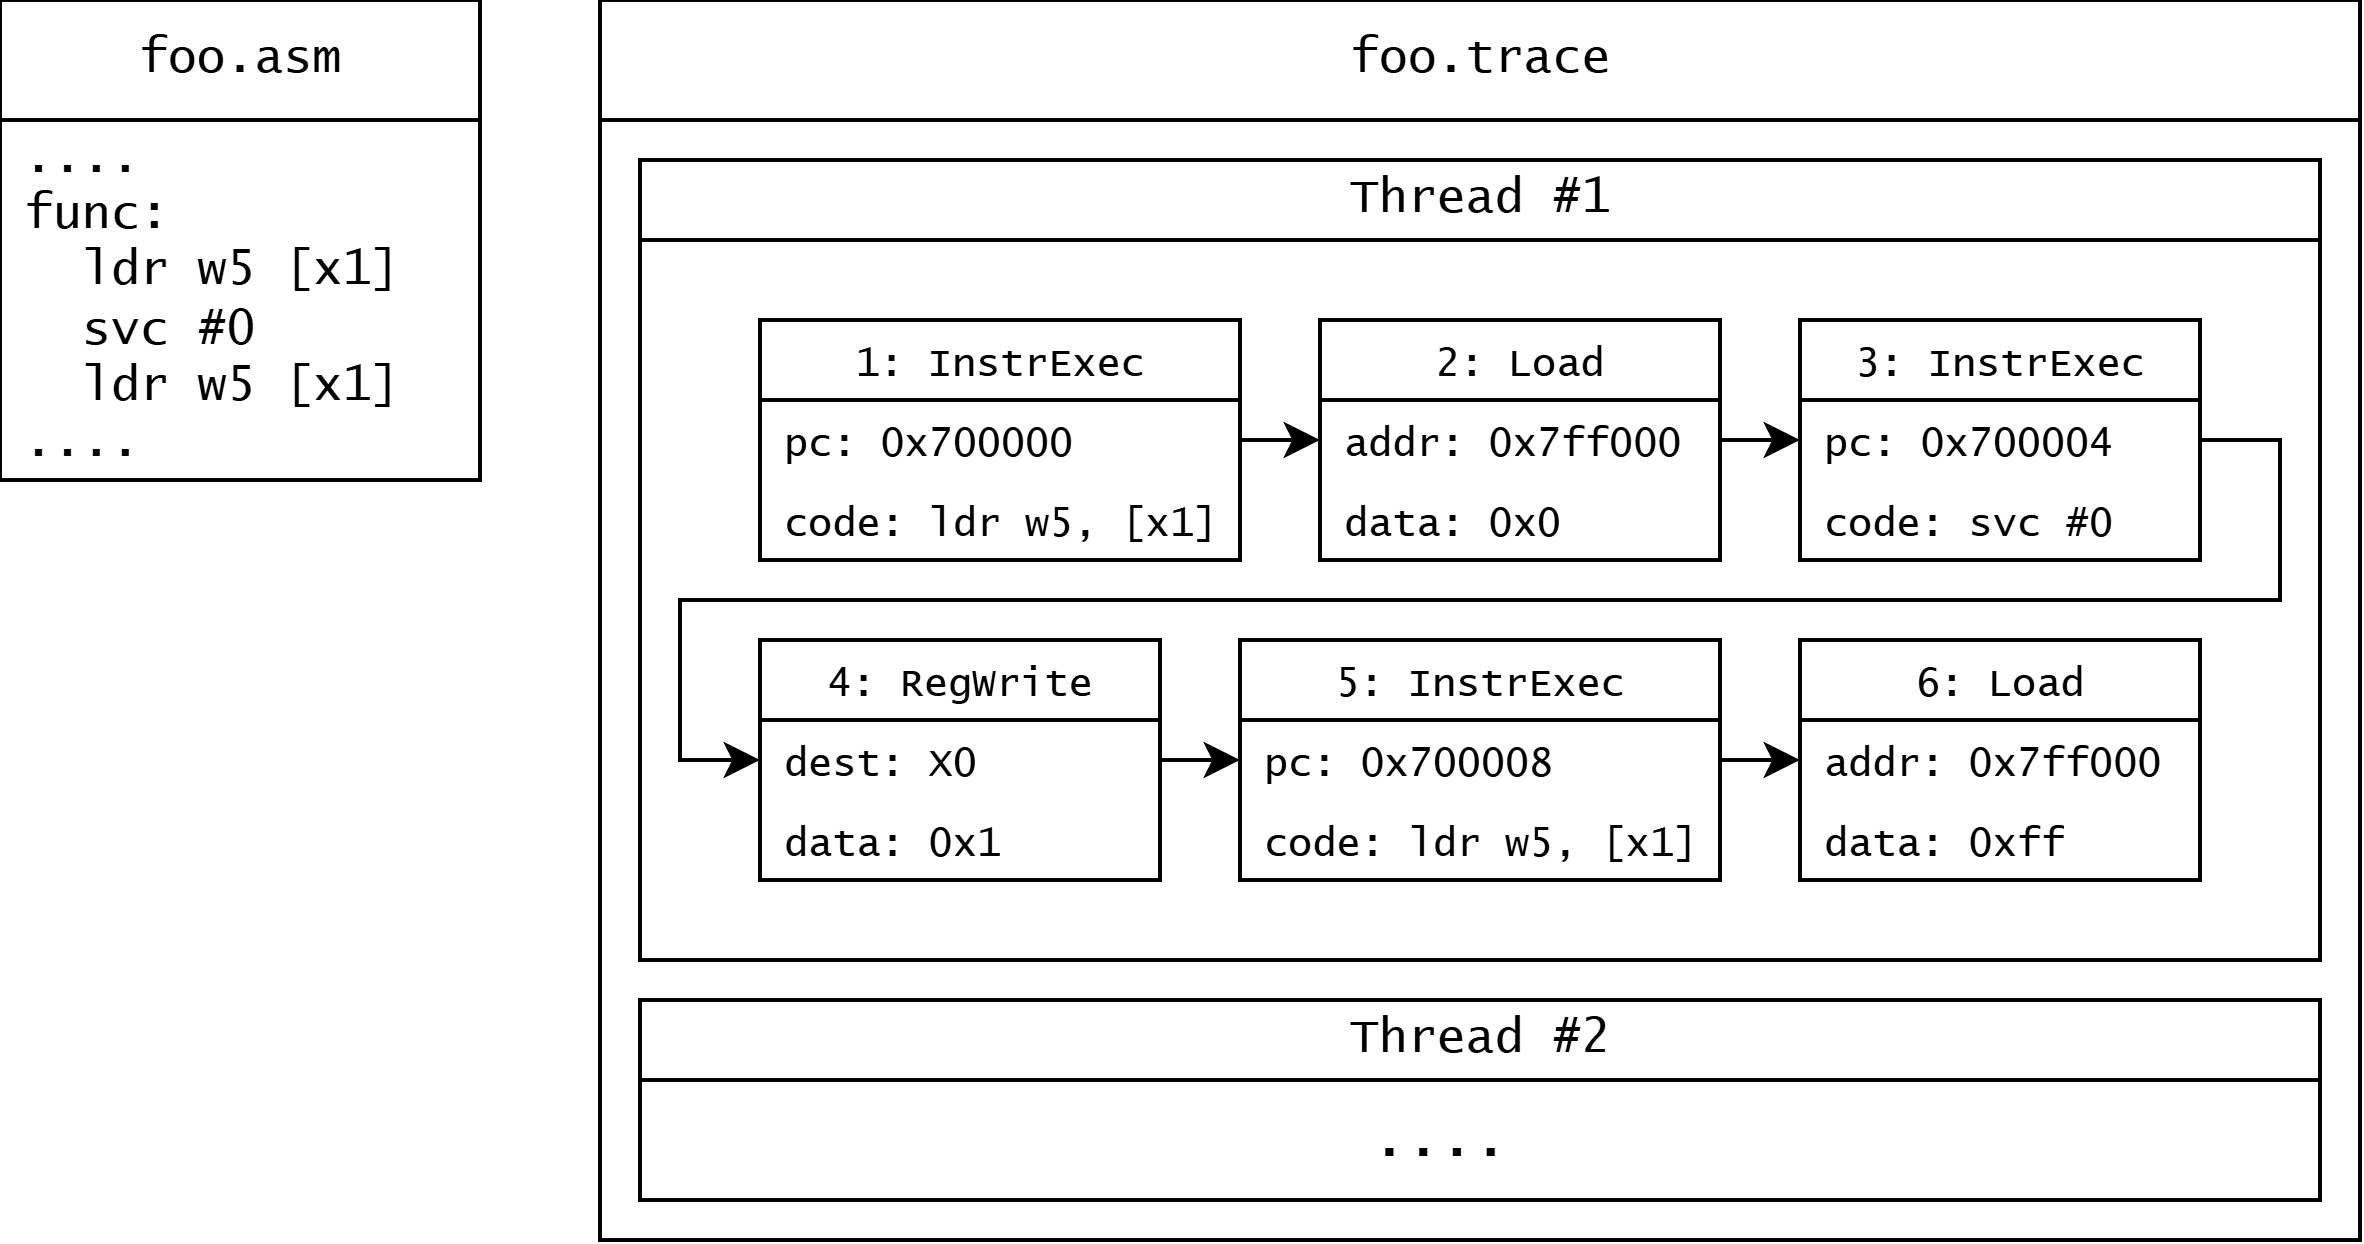
\includegraphics[width=0.8\linewidth]{pics/trace_example.drawio.png}
    \caption{Пример трассы исполнения.}
    \label{fig:trace_example}
\end{figure}

При анализе трасс исполнения часто используются симуляторы \cite{nocua_gem5_trace_driven,synchrotrace}. В таких случаях в состояние симулятора пробрасываются данные из трассы, для рассматриваемых трасс это: начальное регистровое состояние, коды инструкций, данные для чтений из памяти, новые значения регистров общего назначения. При этом зачастую потоки управления и данных симулятора проверяются на соответствие трассе для детектирования ошибок симуляции или невалидных трасс. Такой подход называется симуляцией по трассе.

Описанные особенности трасс исполнения и их обработки позволяют существенно модифицировать записанные сценарии и получать валидные трассы для дальнейшей обработки: можно изменить или добавить необходимые записи для коррекции потоков управления и данных. На рис. \ref{fig:trace_example_modified} приведен пример модифицированной трассы исполнения. Измененные данные выделены красным цветом.

\begin{figure}[h!]
    \centering
    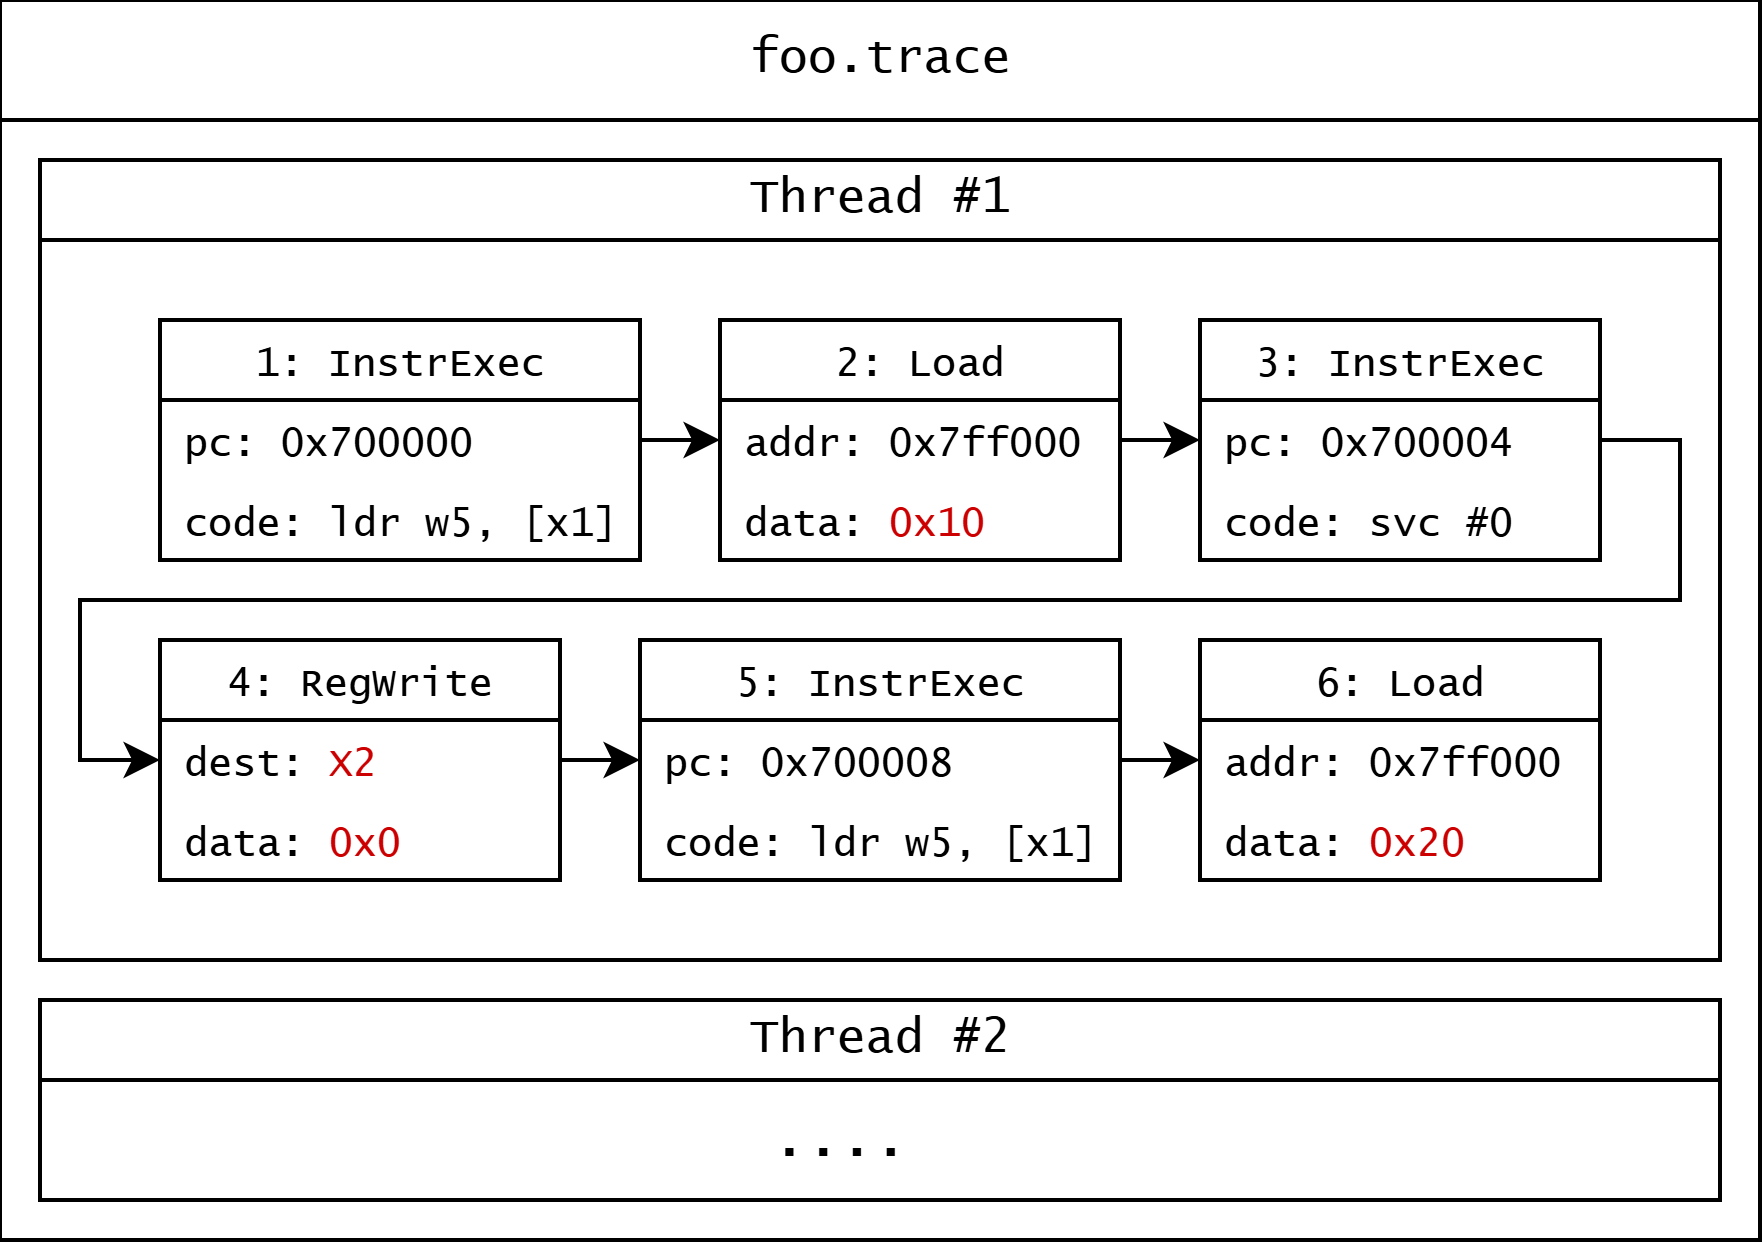
\includegraphics[width=0.6\linewidth]{pics/trace_example_modified.drawio.png}
    \caption{Пример модифицированной трассы исполнения.}
    \label{fig:trace_example_modified}
\end{figure}

\subsection{Репрезентативность трасс} \label{sec:representativeness}

Для оценки репрезентативности трасс обычно сличаются целевые метрики сценариев исполнения и метрики, получаемые при анализе трасс, снятых с этих сценариев. Значения могут расходиться по разным причинам: трассировка может влиять на поведение приложения; используемая модель или методы анализа трасс могут искажать получаемые значения; на исследуемую нагрузку могут влиять внешние факторы.

Как уже было упомянуто ранее, данная работа сфокусирована на использовании трасс исполнения для анализа производительности разрабатываемых платформ. Поэтому основными целевыми метриками являются значения микроархитектурных счетчиков. Для оценки репрезентативности сличаются счетчики, снятые с трассируемого приложения, и счетчики, полученные от используемой модели (сконфигурированной для симуляции трассируемой системы).

При обработке некоторых записей трассы исполнения симулятором или другой моделью появляется необходимость компенсации состояния модели. Пример: из памяти прочитано новое значение, которое ранее не наблюдалось -- требуется модификация памяти симулятора для корректного продолжения работы. Подобные изменения состояния модели производятся посредством исполнения дополнительного кода (далее -- компенсационный код), что может существенно искажать собираемые метрики. Более того, компенсационный код фиксирован для каждой инструкции приложения -- единожды произошедшая при симуляции инструкции трассы компенсация приводит к добавлению компенсационного кода для \textbf{всех} инструкций трассы, отвечающих той же инструкции приложения. Поэтому репрезентативность трасс исполнения существенно зависит от компенсаций, требуемых при обработке.

Подробно методология сбора микроархитектурных метрик и оценки репрезентативности трасс в данной работе рассмотрена не будет. Однако будут приведены метрики, используемые для предварительной оценки качества получаемых трасс.

\subsection{Виртуальное адресное пространство}

Большинство современных компьютерных систем поддерживает виртуализацию адресного пространства \cite{arm_memory_management}. Данная технология позволяет отображать (транслировать) адреса оперативной памяти, используемые кодом (виртуальные адреса) в адреса аппаратуры (физические адреса). Такой подход позволяет запускать множество приложений изолированно в одинаковой среде исполнения. Виртуальные адреса приложений могут пересекаться, однако при обращении к памяти будут использованы разные физические адреса. Создание карты трансляции адресов осуществляет операционная система по запросам приложений и загрузчиков.

При этом трансляция адресов обычно происходит постранично: виртуальное адресное пространство разбивается на непрерывные блоки одинакового размера (виртуальные страницы), последовательные адреса внутри одного блока отображаются в последовательные физические адреса (адреса физической страницы). Размер страницы - очень важный параметр системы, напрямую влияющий на производительность. Уменьшение размера страницы приводит к замедлению трансляции адресов, а увеличение - к большему расходу памяти. Типовые размеры страниц для современных систем: 4096, 16384 и 65536 байт.

К другим настройкам адресации можно отнести расположение запрещенных областей виртуального адресного пространства - областей, использование которых пользовательским кодом запрещено или ограничено. Такие области могут быть заняты данными операционной системы, зарезервированы для будущих расширений, запрещены для детектирования ошибок адресации (null page). Подобные области могут быть доступны из пользовательского кода только на чтение или недоступны вовсе.

Также многие современные системы имеют ограничения на создание отображений c правами на исполнение и запись (WX права) для повышения безопасности \cite{ye_executable_stack,openbsd_kernel_wx}.

\clearpage

\subsection{Цель работы}

Трассы исполнения могут быть использованы для анализа производительности еще не выпущенных платформ. Однако, описанные особенности виртуального адресного пространства существенно усложняют подобный анализ в случае, если настройки адресации разрабатываемой платформы отличаются от настроек адресации платформы, на которой трассы были записаны (исходные настройки адресации). Это мотивирует разработку решения для модификации образов памяти затрассированных сценариев путем изменения трасс исполнения. Заметим, что данная задача сводится к задаче перемещения областей образов памяти трасс в соответствии с новыми ограничениями.

\vspace{0.3cm}

{\bf Цель работы:} Разработать решение, позволяющее перемещать области образов памяти трассируемых сценариев в соответствии с ограничениями, обусловленными настройками адресации разрабатываемой платформы.

\vspace{0.3cm}

{\bf Задачи:}

\begin{itemize}
    \item Разработать модификатор трасс исполнения, перемещающий области образа памяти в соответствии с ограничениями, обусловленными новыми настройками адресации.
    \item Протестировать работоспособность модификатора трасс на целевых трассах заказчика.
    \item Оценить влияние модификаций на репрезентативность трасс исполнения.
\end{itemize}

Работа будет осуществляться в рамках проекта для сбора и анализа трасс исполнения. Будут использованы некоторые компоненты проекта, внешние по отношению к разрабатываемому решению: функциональный симулятор целевой архитектуры, библиотека для чтения и записи трасс исполнения.

\clearpage
 %% Введение
    \section{Обзор существующих решений}

В данной главе будут рассмотрены существующие решения в области переноса кода и данных.

\subsection{Позиционно-независимый код}

Позиционно независимый код (Position Independent Code, \gls{pic}) - это код, который может быть размещен по любому адресу. PIC библиотека или приложение (\glsdisp{module}{модуль}) напрямую не использует фиксированные адреса и для доступа к коду и данным использует относительные смещения или таблицу глобальных смещений (Global Offset Table, \gls{got}) и таблицу связывания процедур (Procedure Linkage Table, \gls{plt}). PIC модули могут быть загружены по любым адресам, что позволяет использовать их с технологией рандомизации адресного пространства (Address Space Layout Randomization, \gls{aslr}) и существенно упрощает динамическое связывание библиотек.

\begin{figure}[h!]
    \centering
    \begin{minipage}{0.4\textwidth}
        \centering
        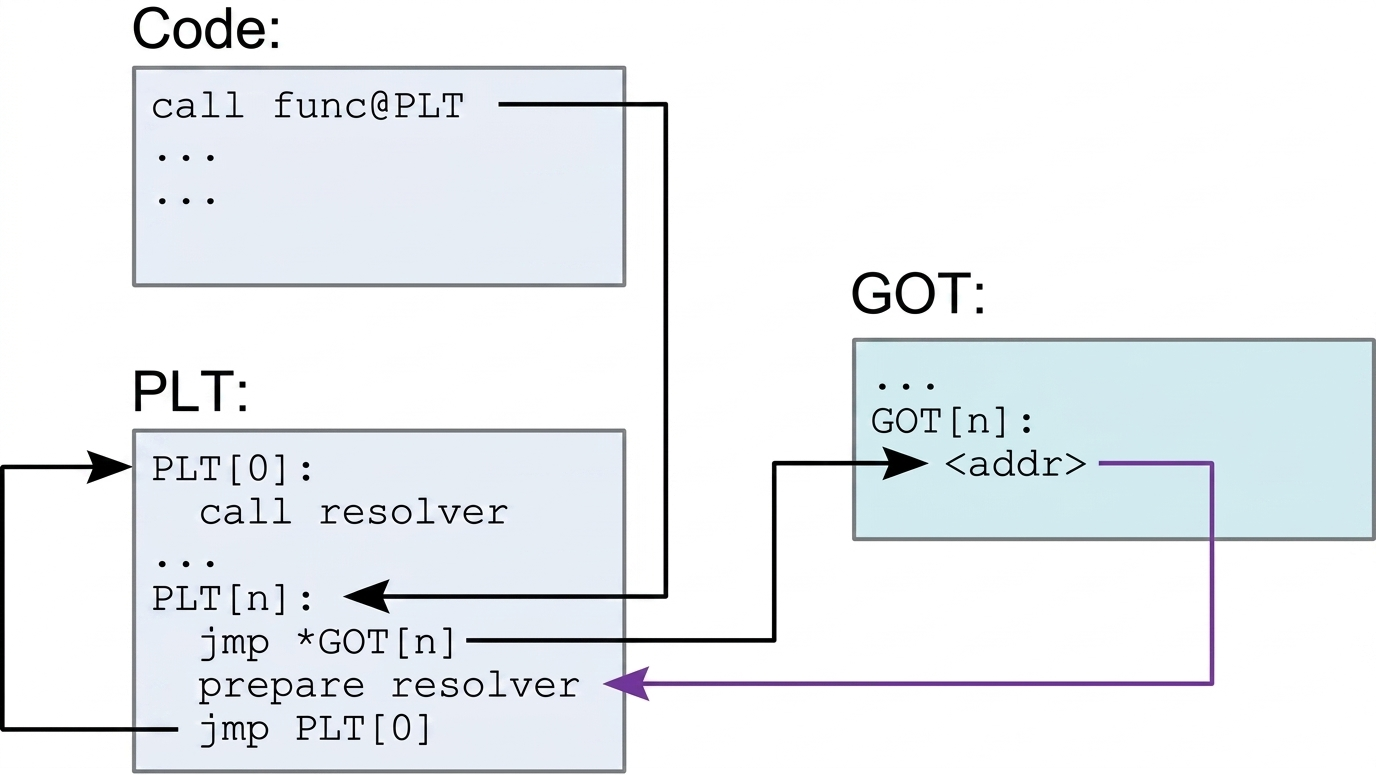
\includegraphics[width=\linewidth]{pics/bendersky_pic_in_shared_libs_plt1.png}
        \caption{Схема работы PLT: первый вызов процедуры \cite{bendersky_pic_in_shared_libs}.}
        \label{fig:bendersky_pic_in_shared_libs_plt1}
    \end{minipage}
    \hspace{2cm}
    \begin{minipage}{0.4\textwidth}
        \centering
        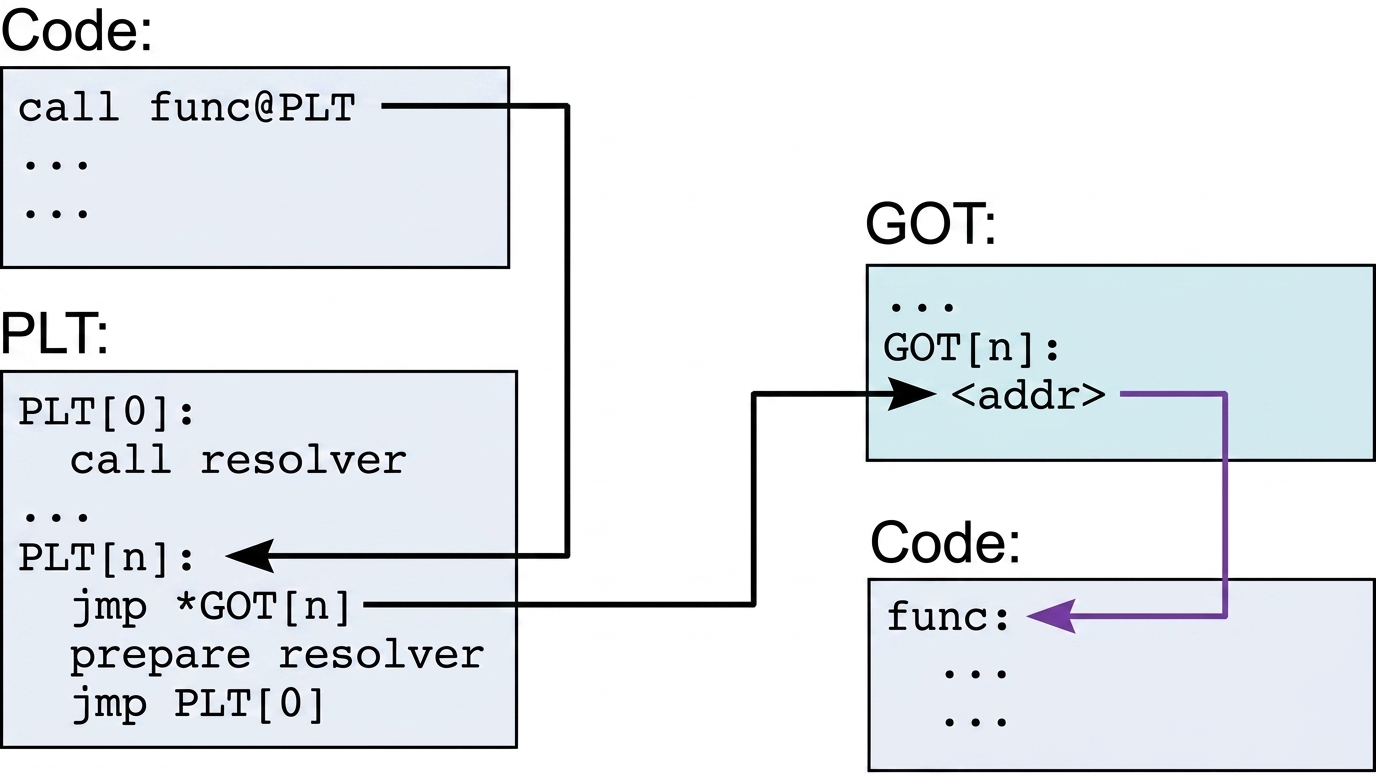
\includegraphics[width=\linewidth]{pics/bendersky_pic_in_shared_libs_plt2.png}
        \caption{Схема работы PLT: последующие вызовы \cite{bendersky_pic_in_shared_libs}.}
        \label{fig:bendersky_pic_in_shared_libs_plt2}
    \end{minipage}
\end{figure}

Данная технология используется на целевой платформе, что упрощает модификацию затрассированного образа памяти, так как при переносе PIC сегмента целиком, относительная адресация внутри сегмента будет работать как в оригинальном сценарии (смещения между символами сегмента не изменятся). Однако исходные адреса кода и данных могут остаться на стеке, в куче и GOT. Так же относительная адресация внутри одного модуля перестанет корректно работать в случае переноса сегментов модуля с разными смещениями.

\subsection{Компоновщики}

В ходе статической компоновки из набора объектных файлов и статических библиотек создается один готовый исполняемый файл или библиотека (статическая или динамическая). Сегменты кода и данных входных файлов объединяются, происходит разрешение символов, с помощью данных из таблиц перемещений производятся замены адресов и смещений в коде и данных на финальные. Результирующий модуль содержит код и данные входных объектных файлов и статических библиотек, все символы разрешаются при компоновке.

Статическая компоновка позволяет осуществлять интер-модульные оптимизации (post-link optimizations) и уменьшает вычислительные расходы на загрузку приложения так как связывание происходит один раз при компоновке исполняемого файла. При этом данный метод может существенно увеличивать нагрузку на подсистему памяти во время исполнения множества приложений с одинаковыми зависимостями, поскольку код и данные каждой статической библиотеки будут продублированы в каждом приложении.

При динамической компоновке разрешение символов динамических библиотек откладывается до их загрузки (или даже непосредственно до использования). Компоновщик проверяет, что все внешние символы экспортируются какой-то из динамических библиотек, записывает имена динамических библиотек и их символов, создает GOT и PLT. Адреса динамически связываемых символов разрешаются во время их загрузки или использования специально сгенерированным кодом с помощью таблиц перемещений.

Динамическая компоновка позволяет ОС единожды загрузить динамическую библиотеку и предоставить ее код и данные в общее пользование всем зависимым процессам. Применение данного подхода позволяет существенно снижать потребление памяти современных систем. При этом динамическое связывание происходит непосредственно во время исполнения приложения, что приводит к дополнительным вычислительным расходам.

Следует отметить, что в обоих сценариях используются подготовленные компилятором и компоновщиком таблицы перемещений, т.е. локации заменяемых адресов и смещений известны.

\subsection{Компиляторы}

При однопроходной или двухпроходной компиляции адреса целевых меток кода могут быть неизвестны на момент генерации инструкций перехода на эти метки. Часто для корректного формирования инструкций перехода используется метод отложенного связывания (backpatching). При таком подходе инструкции перехода, для которых неизвестны смещения до целевых меток, генерируются с незаполненными смещениями и локации таких инструкций помещаются в список для дальнейшего исправления. Когда расположение целевой метки становится известным (например после обработки всей единицы трансляции), смещения зависимых инструкций заполняются корректными значениями.

Данный подход позволяет генерировать код без дополнительных полных проходов по промежуточному представлению. В качестве недостатков этого метода можно выделить затраты памяти на хранение вспомогательной информации и потенциальное усложнение оптимизаций, переставляющих участки кода.

\subsection{Сборщики мусора ВМ}

Среды выполнения многих языковых виртуальных машин (\gls{vm}) включают сборщики мусора, которые помимо освобождения неиспользуемой памяти могут перемещать используемые данные для решения проблемы фрагментации памяти, улучшения кеш-локальности и других оптимизаций.

Одним из наиболее распространенных семейств алгоритмов сборки мусора является семейство трассирующих сборщиков мусора. Зависимости между объектами, расположенными в памяти виртуальной машины, можно представить в виде направленного графа (граф объектов). Вершины графа - объекты, ребра - ссылки между объектами. Для определения того, какие объекты можно удалять и как обновлять ссылки на еще используемые объекты при их перемещении, осуществляются обходы графа из "корневых"\, объектов: объектов расположенных на регистрах и стеке ВМ, глобальных объектов, и т. д. Объекты, недостижимые из корневых объектов, можно очищать. А для перемещаемых объектов в ходе такого обхода собираются все ссылки, которые необходимо обновить.

Описанная методология позволяет эффективно освобождать память (в том числе очищать объекты, использующие циклические ссылки) и осуществлять дефрагментацию используемой памяти.

\subsection{Динамическое восстановление вырезанных таблиц перемещений}

Старые бинарные выпуски библиотек могут являться позиционно зависимыми, что делает системы, которые используют подобные версии библиотек уязвимыми для атак повторного использования кода (code reuse attacks). В \cite{dyn_rec_of_stripped_reloc_info} представлен метод динамического восстановления таблиц перемещений для позиционно зависимых библиотек, из которых была вырезана данная информация. Технология применяется для частичной рандомизации адресов загрузки позиционно зависимых библиотек, что повышает безопасность уязвимых систем.

При загрузке позиционно зависимой библиотеки код загружается по случайным адресам, а адреса, зарезервированные для кода библиотеки (старые адреса кода), запрещаются для использования через механизмы операционной системы, такие как mmap. При доступе к старым адресам кода производится обработка системного исключения, в ходе которой анализируется паттерн обращения и либо осуществляется замена адреса на перемещенный, либо обращение помечается как потенциально вредоносное и выводится ошибка.

\begin{figure}[h!]
    \centering
    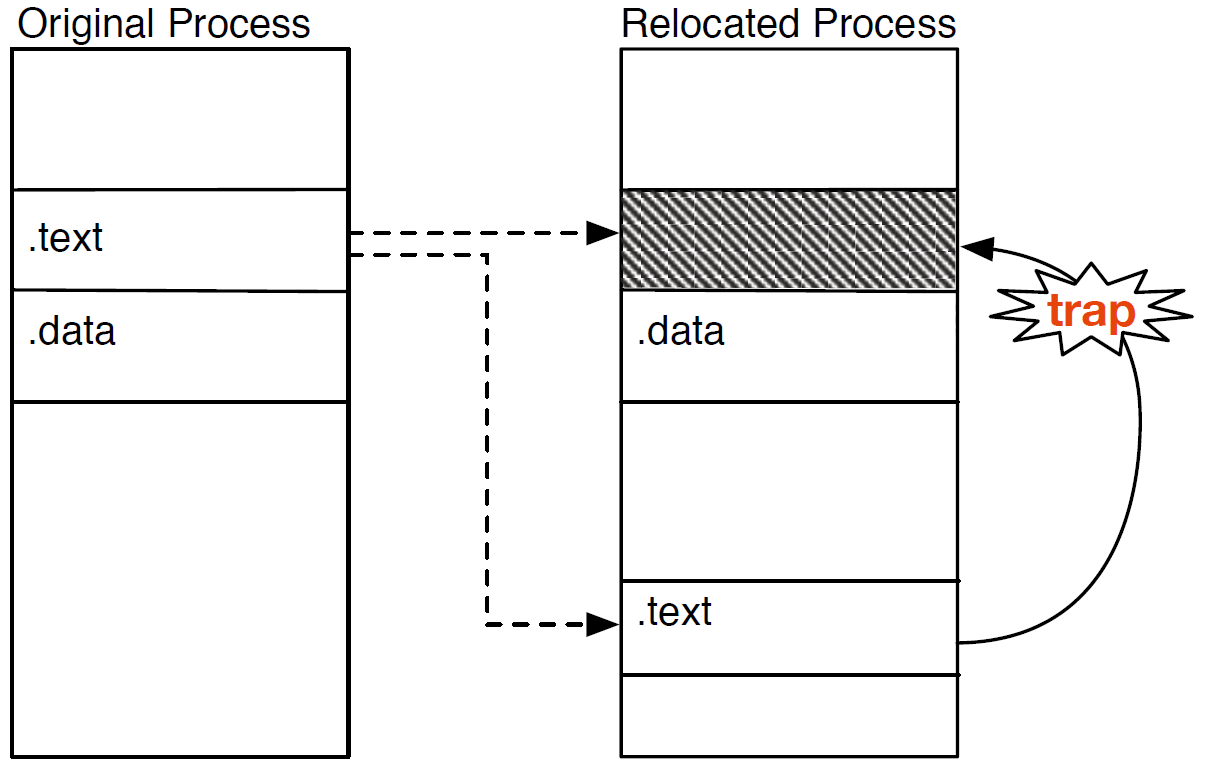
\includegraphics[width=0.6\linewidth]{pics/dyn_rec_of_stripped_reloc_info.png}
    \caption{Схема загрузки позиционно зависимых библиотек с частичной рандомизацией адресов \cite{dyn_rec_of_stripped_reloc_info}}
    \label{fig:dyn_rec_of_stripped_reloc_info}
\end{figure}

\clearpage
 %% Постановка задачи
    \section{Решение задачи}

В данной главе будет рассмотрено решение поставленной задачи. Решение разработано на языке программирования C++.

\subsection{Архитектура решения}

Общая схема решения представлена на рис. \ref{fig:solution_overview}.

\begin{figure}[h!]
    \centering
    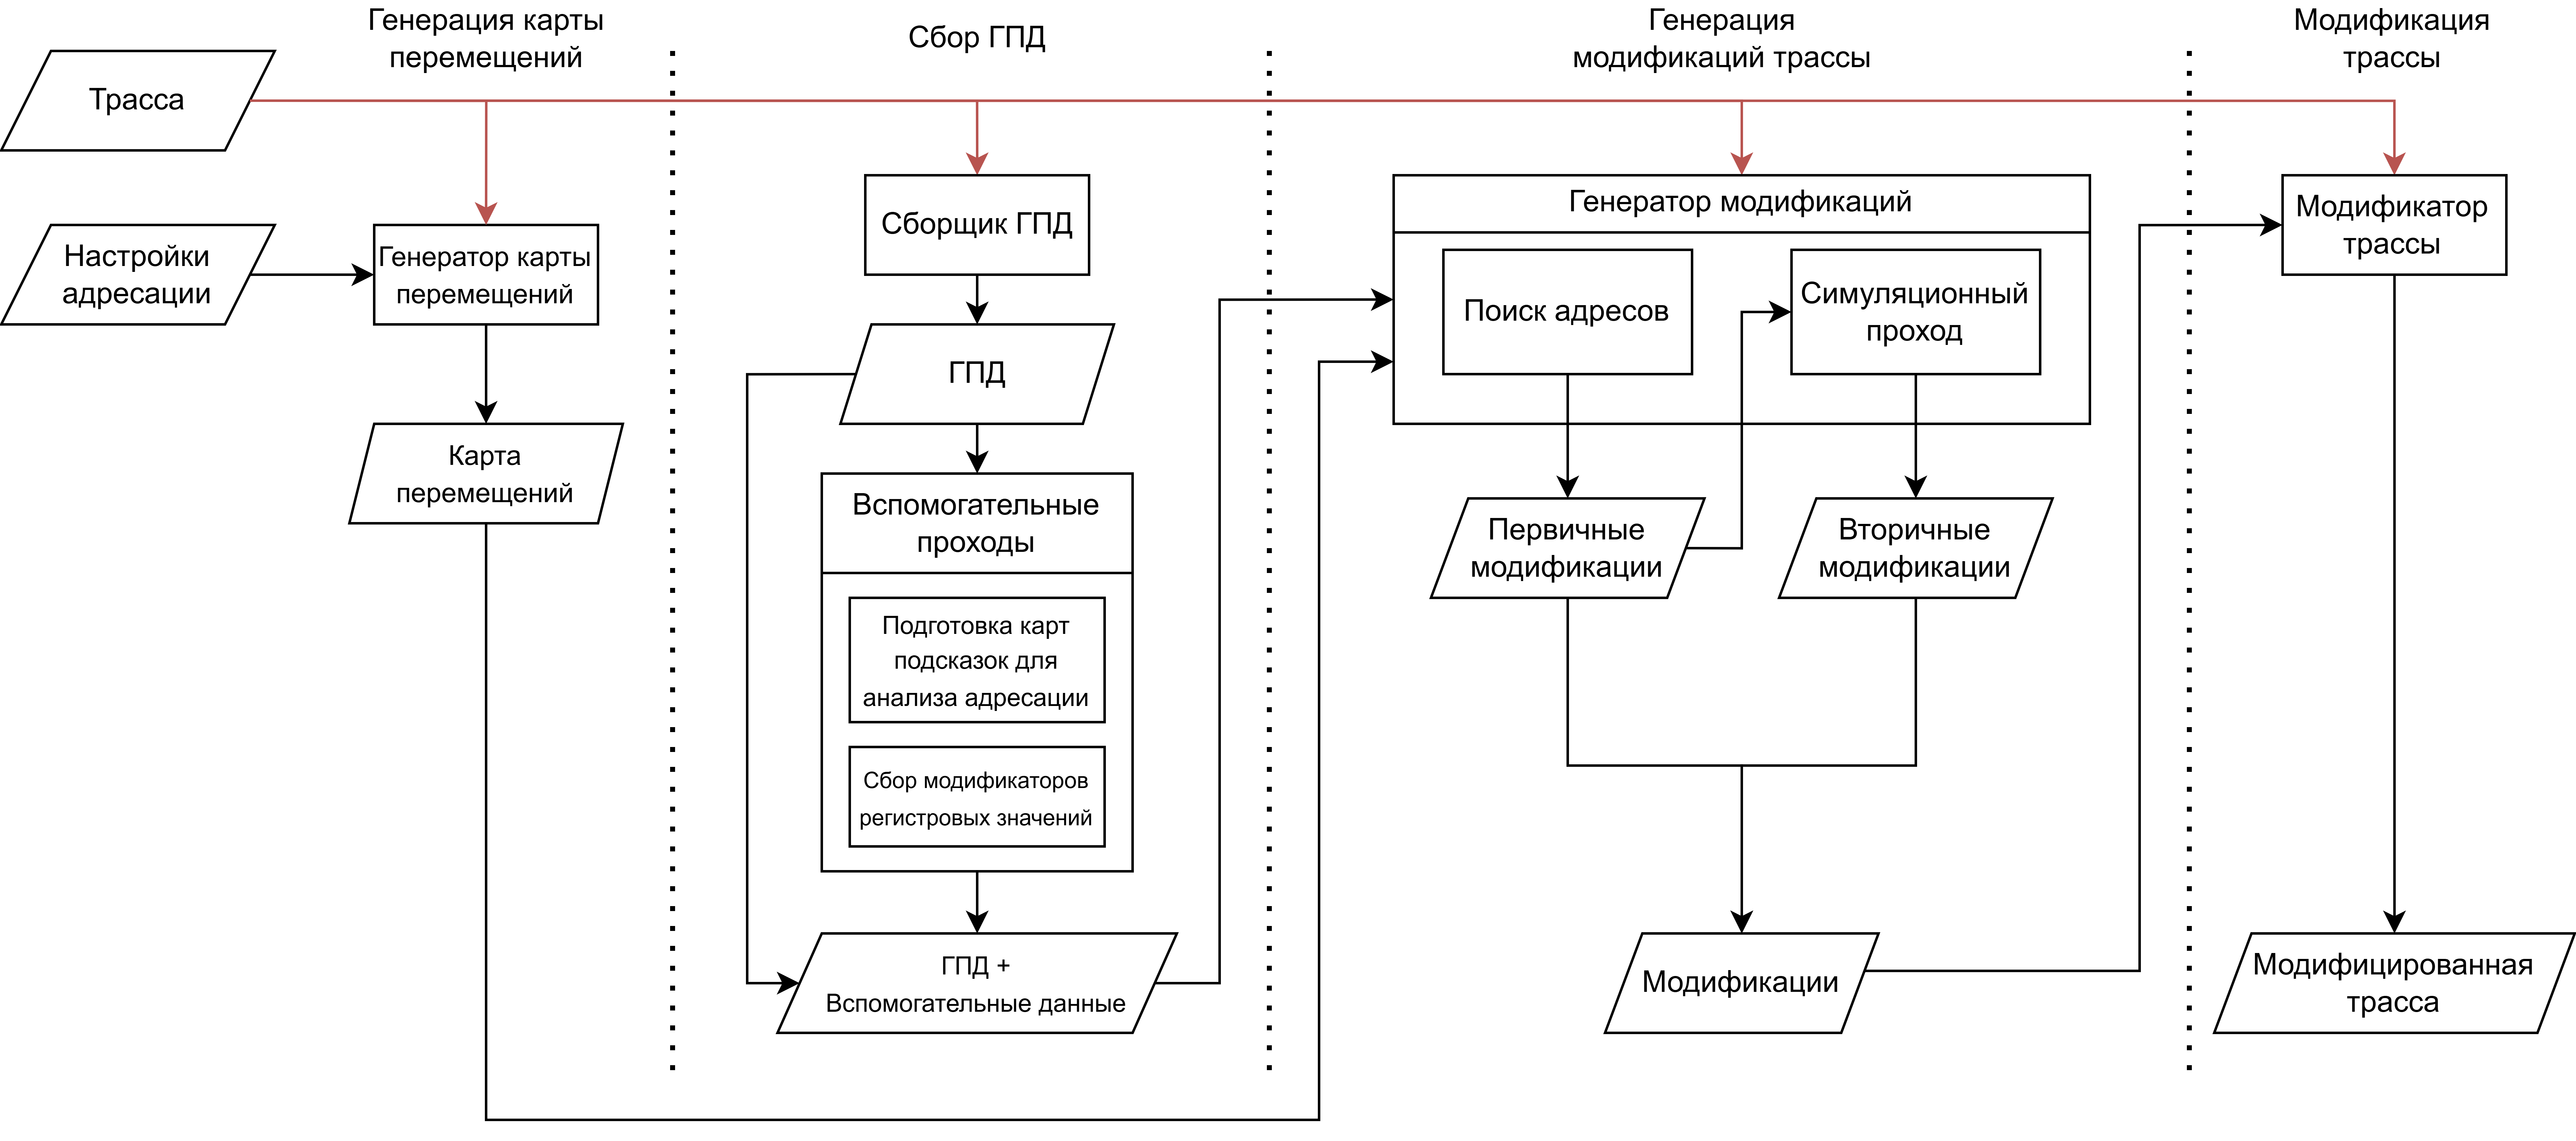
\includegraphics[width=\linewidth]{pics/solution_overview.drawio.png}
    \caption{Общая схема решения.}
    \label{fig:solution_overview}
\end{figure}
\FloatBarrier

Обработка трассы происходит в четыре стадии:

\begin{enumerate}
    \item Генерация карты перемещений

    На этой стадии генерируется карта перемещений областей памяти, удовлетворяющая новым ограничениям, обусловленным изменением настроек адресации.

    \item Сбор графа потока данных (\gls{dfg})

    На данной стадии осуществляется симуляционный проход по трассе, в ходе которого собирается ГПД. Затем осуществляется ряд обходов графа, в ходе которых собирается вспомогательная информация, размечающая его.

    \item Генерация модификаций трассы

    Генерация происходит в два этапа:

    \begin{enumerate}
        \item Поиск адресов на ГПД и генерация первичных модификаций

        \item Симуляционный проход по модифицированной трассе и генерация вторичных модификаций
    \end{enumerate}

    \item Запись модифицированной трассы
\end{enumerate}

Генерируемые модификации могут изменять существующие и добавлять новые записи, обеспечивая консистентность выходной трассы. Примеры возможных модификаций были представлены в разделе \ref{sec:execution_traces}. Некоторые модификации могут снижать репрезентативность выходной трассы, так как будут приводить к изменению целевых счетчиков при дальнейшей ее обработке.

\subsection{Генерация карты перемещений}

На данной стадии с трассы собирается карта прав доступа для всех используемых приложением адресов. Далее производится слияние близких областей памяти с разрешенными комбинациями прав доступа. Максимальное расстояние для слияния областей является параметром командной строки. Затем производится перемещение полученных областей памяти в соответствии с новыми ограничениями адресации:

\begin{itemize}
    \item При наличии в исходной карте прав доступа областей с запрещенными комбинациями прав выводится ошибка -- корректное преобразование трассы невозможно.
    \item Области, при слиянии прав доступа которых получится комбинация прав, запрещенная новыми настройками адресации, размещаются на расстоянии, превышающем новый размер страниц памяти.
    \item Также перемещение производится только в области памяти, разрешенные новой конфигурацией.
\end{itemize}

Полученная карта перемещений используется последующими стадиями для анализа адресации и корректной замены адресов. Пример генерации карты перемещений приведен на рис. \ref{fig:reloc_map_example}.

\begin{figure}[h!]
    \centering
    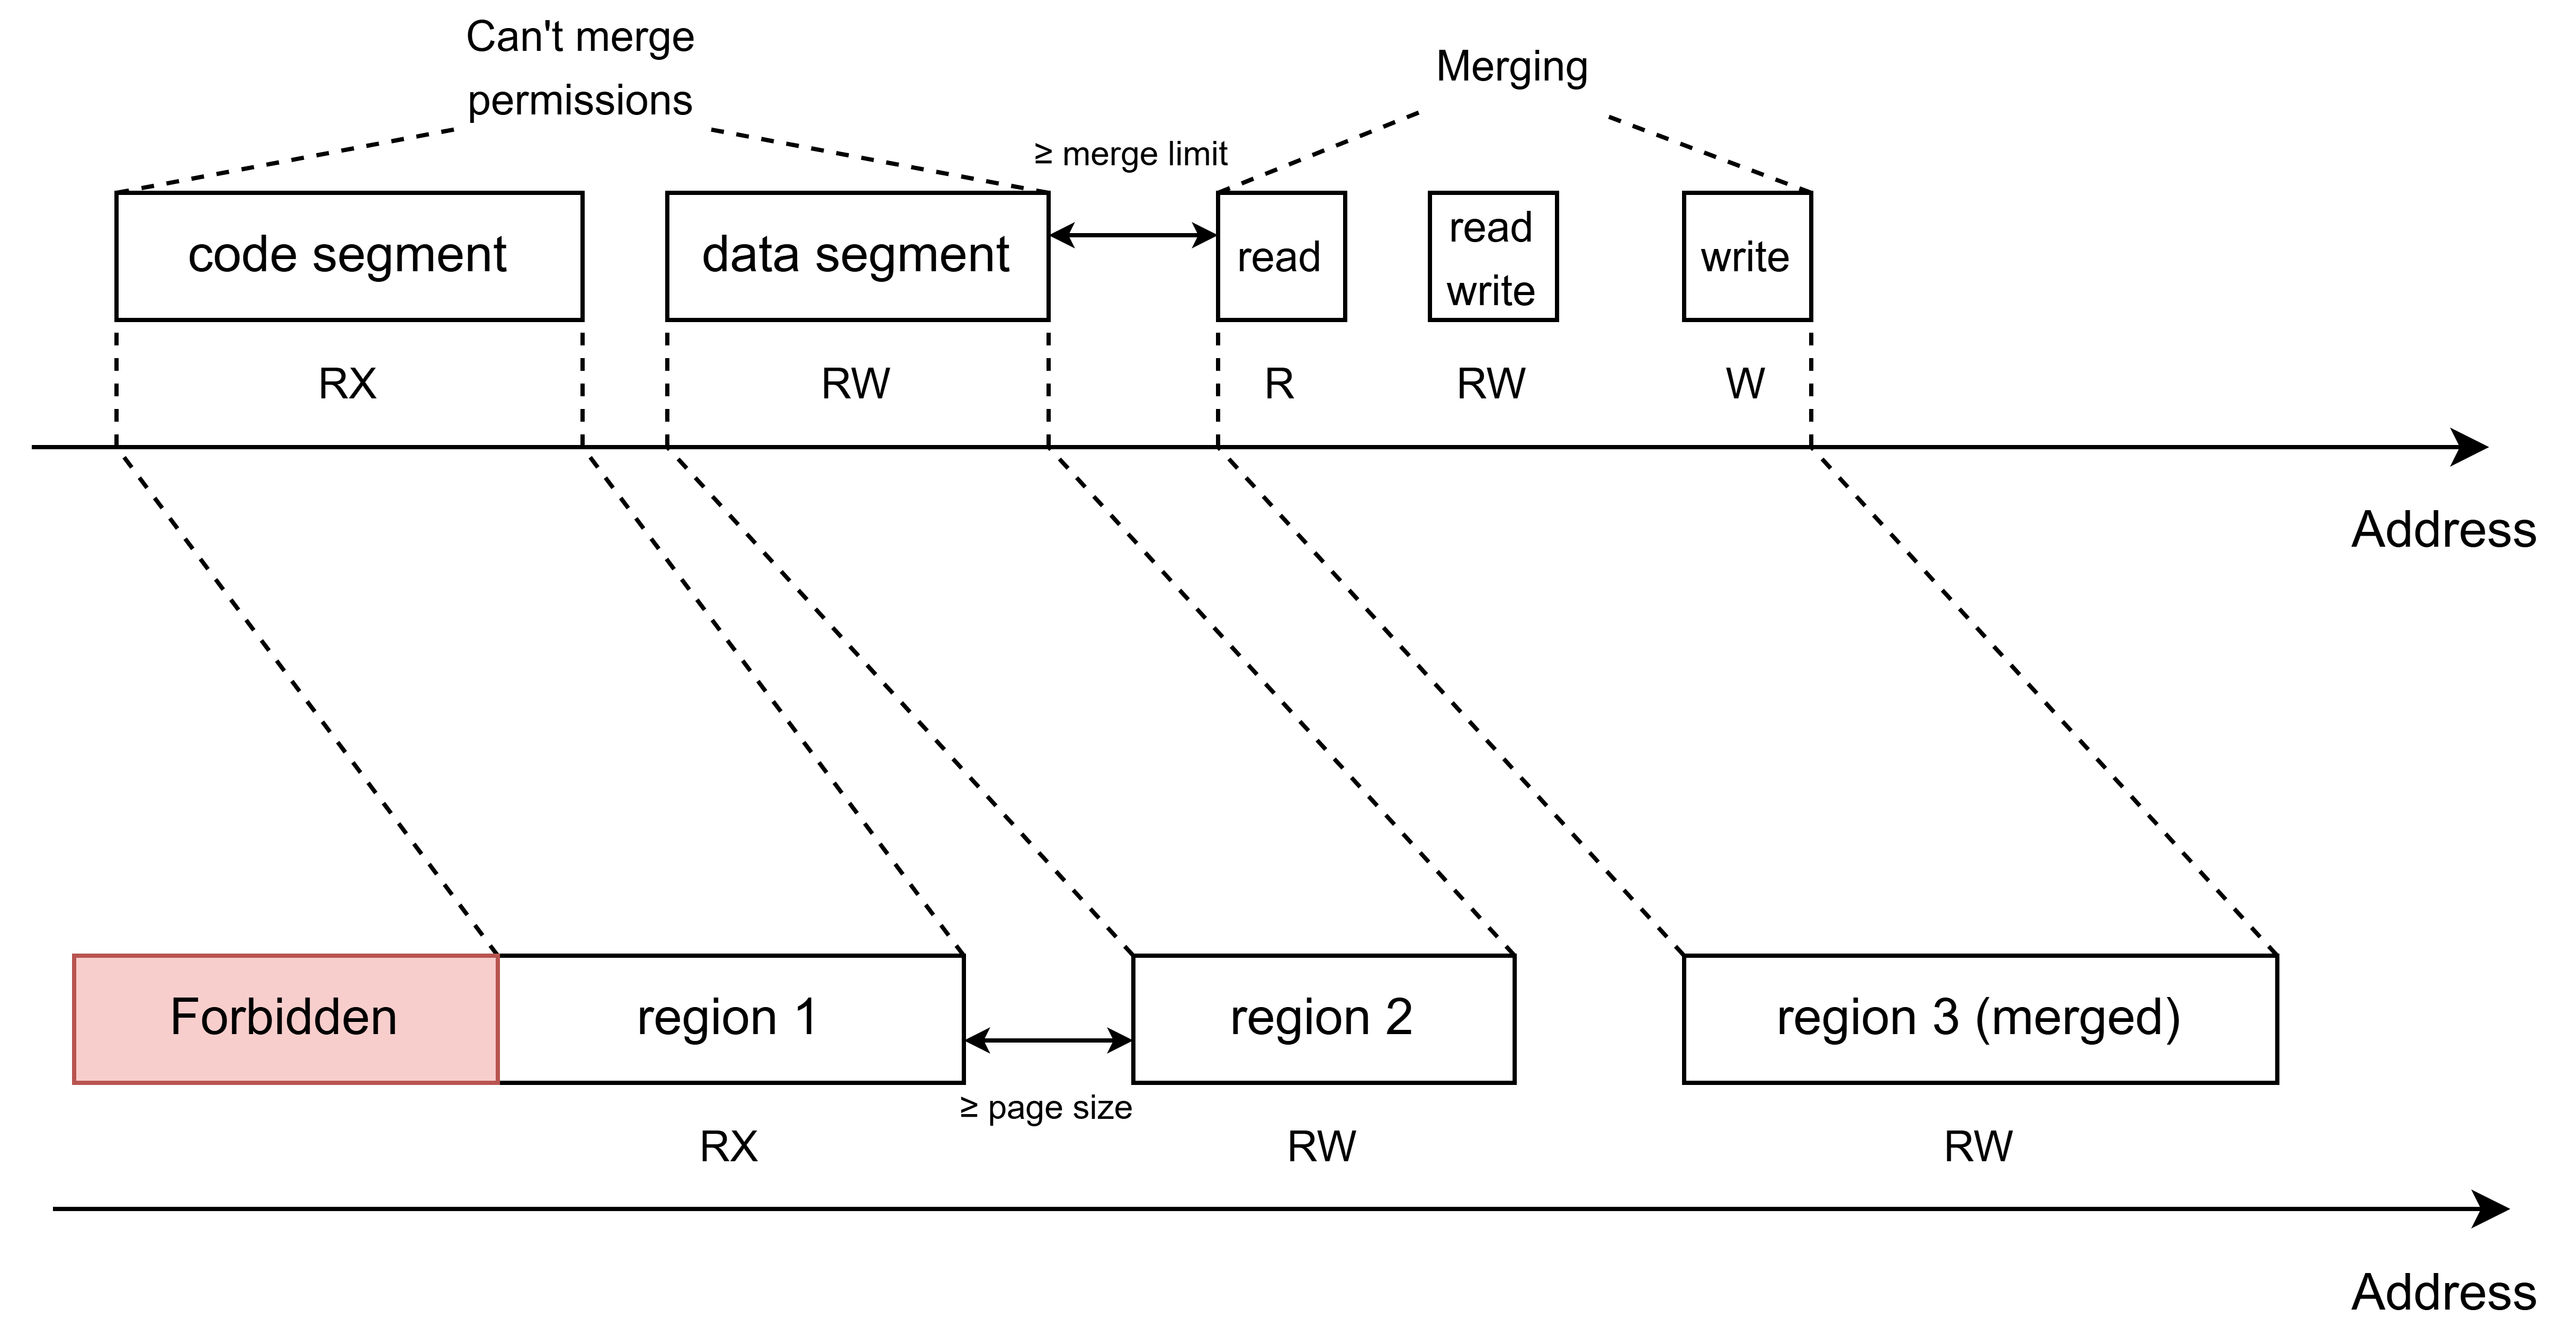
\includegraphics[width=0.9\linewidth]{pics/reloc_map_example.drawio.png}
    \caption{Пример генерации карты перемещений.}
    \label{fig:reloc_map_example}
\end{figure}

\FloatBarrier

\subsection{Сбор графа потока данных} \label{sec:dfg_collection}

Обозначим \gls{dfg_math} - граф потока данных, где $V$ \, - множество вершин графа, $E \subseteq V \times V$ \, - множество ребер графа. Так же обозначим: \gls{edges_subsets} \, - множество всех подмножеств ребер графа. Вершины графа соответствуют отдельным выполнениям инструкций и далее называются инструкциями. Ребра -- зависимости между инструкциями по данным. С каждым ребром ассоциируются значение и локация, по которой данное значение располагалось во время трассировки, например регистр или область памяти. Для представления графа потока данных используется реализация списка смежности из библиотеки boost graph (boost::adjacency\_list) \cite{boost_graph_library,boost_adjacency_list}.

Boost graph позволяет ассоциировать с вершинами и ребрами пользовательские данные. Для инструкций хранятся: номер (уникальный идентификатор) инструкции, адрес инструкции, ее код. Для ребер хранятся: восьми-байтное значение и его локация (уже упомянутые ранее) - в памяти или на регистре общего назначения, модификаторы значения: тип расширения, размеры битовых сдвигов, и т. п. Заметим, что размер значения фиксированный, зависимости по значениям большего размера отображаются с помощью нескольких ребер.

На графе есть вершины, не соответствующие реальным инструкциям (вершина "начальное состояние"\, на рис. \ref{fig:dfg_example}). Будем называть такие вершины \glsdisp{pseudo_source}{псевдо-инструкциями}. Такие вершины всегда являются истоками и используются для отображения зависимостей, не порождаемых отдельными инструкциями, или для добавления вспомогательных зависимостей:

\begin{itemize}
    \item Вершина начального состояния - для зависимостей от начального состояния памяти или начальных значений регистров.

    \item Вершина внешних зависимостей по памяти - для зависимостей по памяти, модифицированной другим потоком или ОС.

    Пример: Из памяти прочитано значение, не соответствующее текущему образу памяти. Данное значение могло быть записано другим потоком или ОС во время системного вызова или обработки системного исключения. На графе данная зависимость будет представлена в виде ребра, выходящего из вершины внешних зависимостей и входящего в инструкцию, прочитавшую новое значение.

    \item Вершина сложных зависимостей по памяти - для зависимостей по памяти от нескольких инструкций.

    В данный момент полноценная поддержка таких зависимостей отсутствует.
\end{itemize}

\begin{figure}[h!]
    \centering
    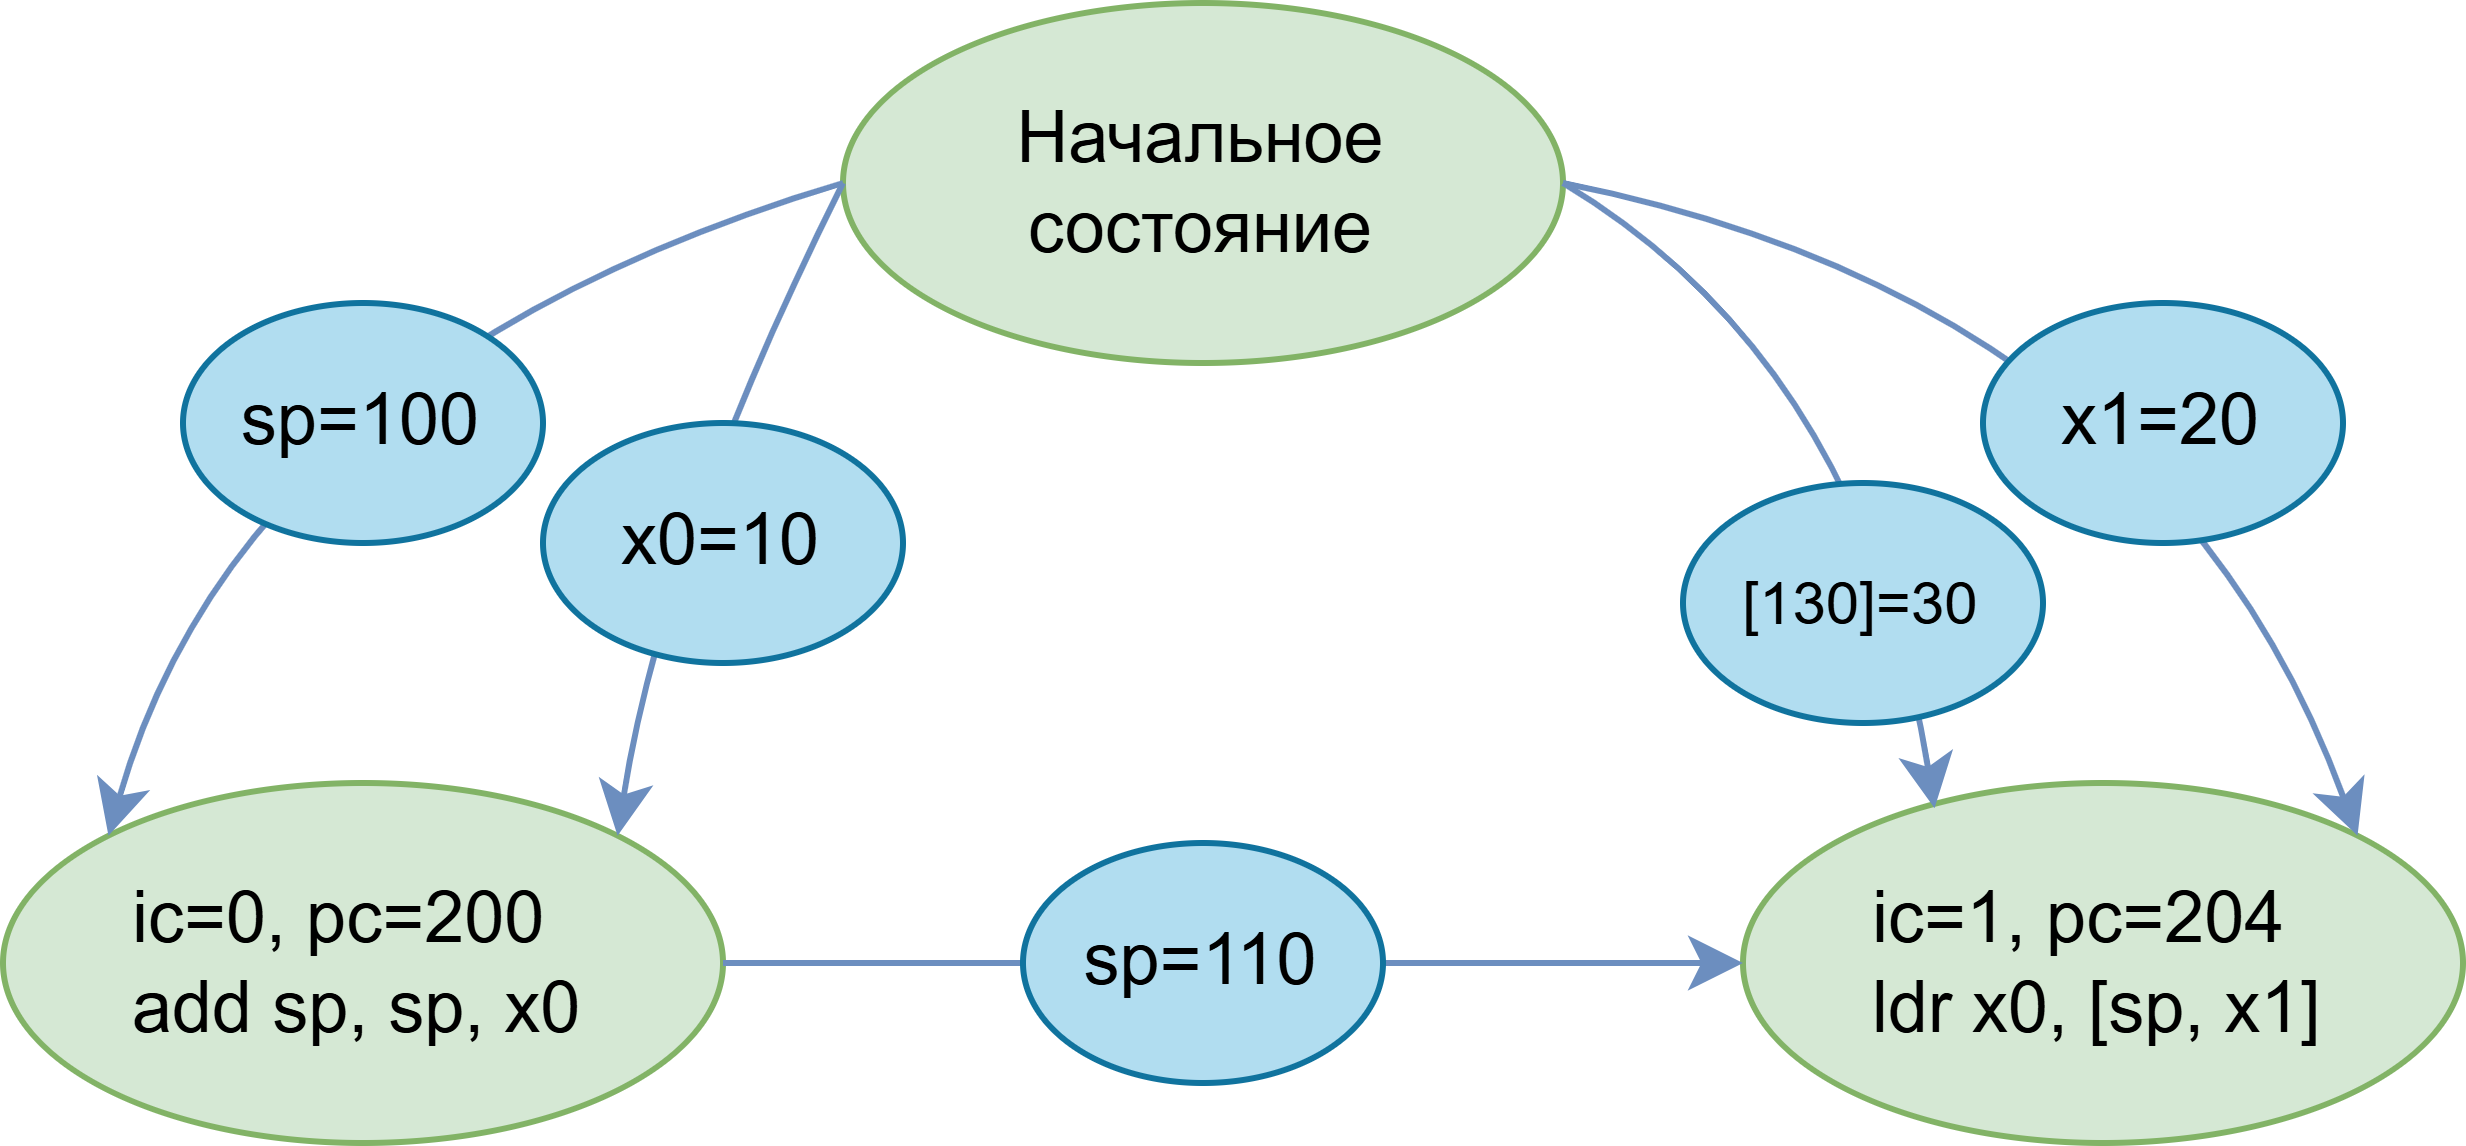
\includegraphics[width=0.7\linewidth]{pics/dfg_example.drawio.png}
    \caption{Пример графа потока данных.}
    \label{fig:dfg_example}
\end{figure}
\FloatBarrier

Сбор графа потока данных начинается с симуляционного прохода по трассе (блок схема алгоритма представлена на рис. \ref{fig:trace_simulation}), в ходе которого собираются:

\begin{itemize}
    \item Граф потока данных.
    \item Данные вершин.
    \item Данные ребер, кроме модификаторов значений (таких как размеры битовых сдвигов и т. п.).
    \item Карта, отображающая идентификаторы инструкций в дескрипторы, с помощью которых осуществляется доступ к вершинам.
    \item Карта зависимостей инструкций от флагов условий.
\end{itemize}

Заметим, что зависимости между инструкциями по флагам условий хранятся отдельно от графа потока данных. Данное решение позволяет разделить разнородные зависимости, что существенно упрощает обработку.

\begin{figure}[h!]
    \centering
    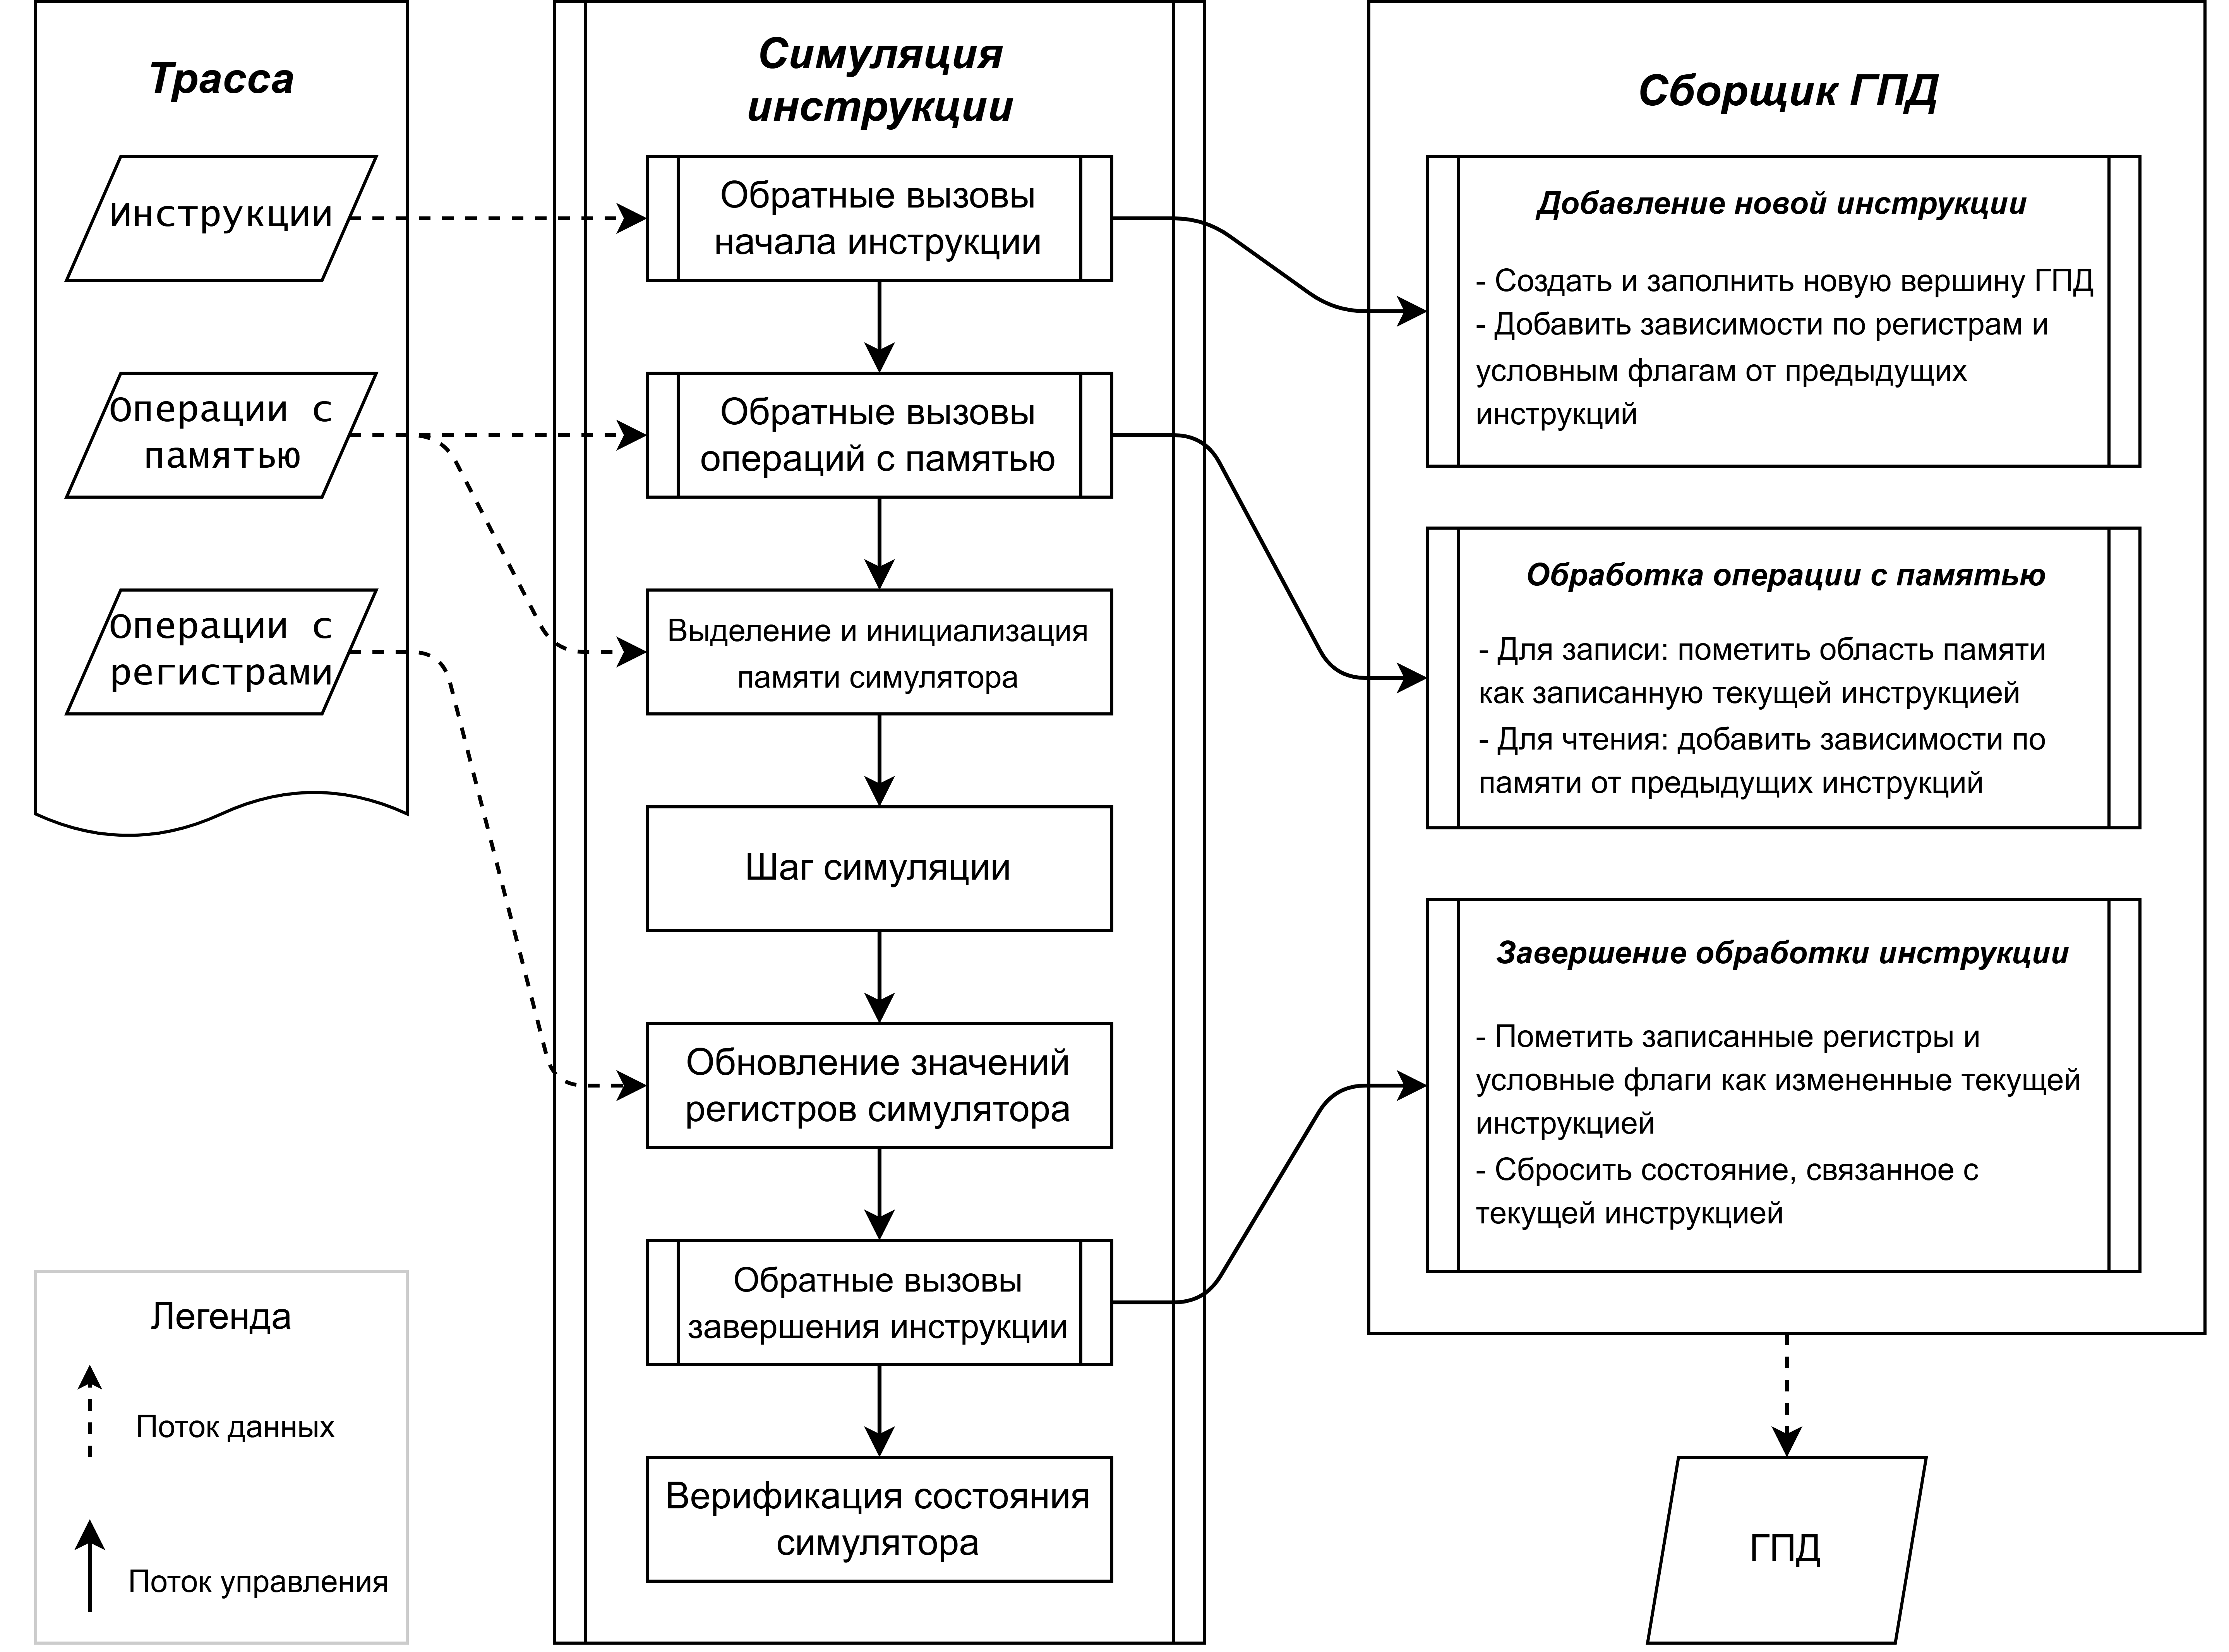
\includegraphics[width=0.8\linewidth]{pics/trace_simulation.drawio.png}
    \caption{Блок схема алгоритма симуляционного прохода по трассе.}
    \label{fig:trace_simulation}
\end{figure}
\FloatBarrier

После симуляционного прохода производится ряд обходов графа, в ходе которых собираются:

\begin{itemize}
    \item Карты подсказок для алгоритмов анализа адресов.
    \item Модификаторы значений для ребер графа.
\end{itemize}

Карты подсказок позволяют получать вспомогательные данные для вершин и ребер графа (примеры фрагментов ГПД и сформированных для них подсказок представлены на рис. \ref{fig:heuristics_hints}):

\begin{itemize}
    \item src\_edge\_hints : $E \rightarrow E$ \, задает порядок обратного обхода графа для алгоритма поиска адресов в ряде краевых случаев. Формируется с помощью набора эвристик.
    \item dst\_edge\_hints : $E \rightarrow 2^E = src\_edge\_hints^{-1}$ \, задает порядок прямого обхода графа для алгоритма поиска адресов в ряде краевых случаев. Задает обратное многозначное отображение для src\_edge\_hints.
    \item base\_edge\_hints : $V \rightarrow E$ \, отображает вершины в соответствующие им входные ребра базовых адресов.
    \item offset\_edge\_hints : $V \rightarrow E$ \, отображает вершины в соответствующие им входные ребра смещений адресов.
\end{itemize}

\begin{figure}[h!]
    \centering
    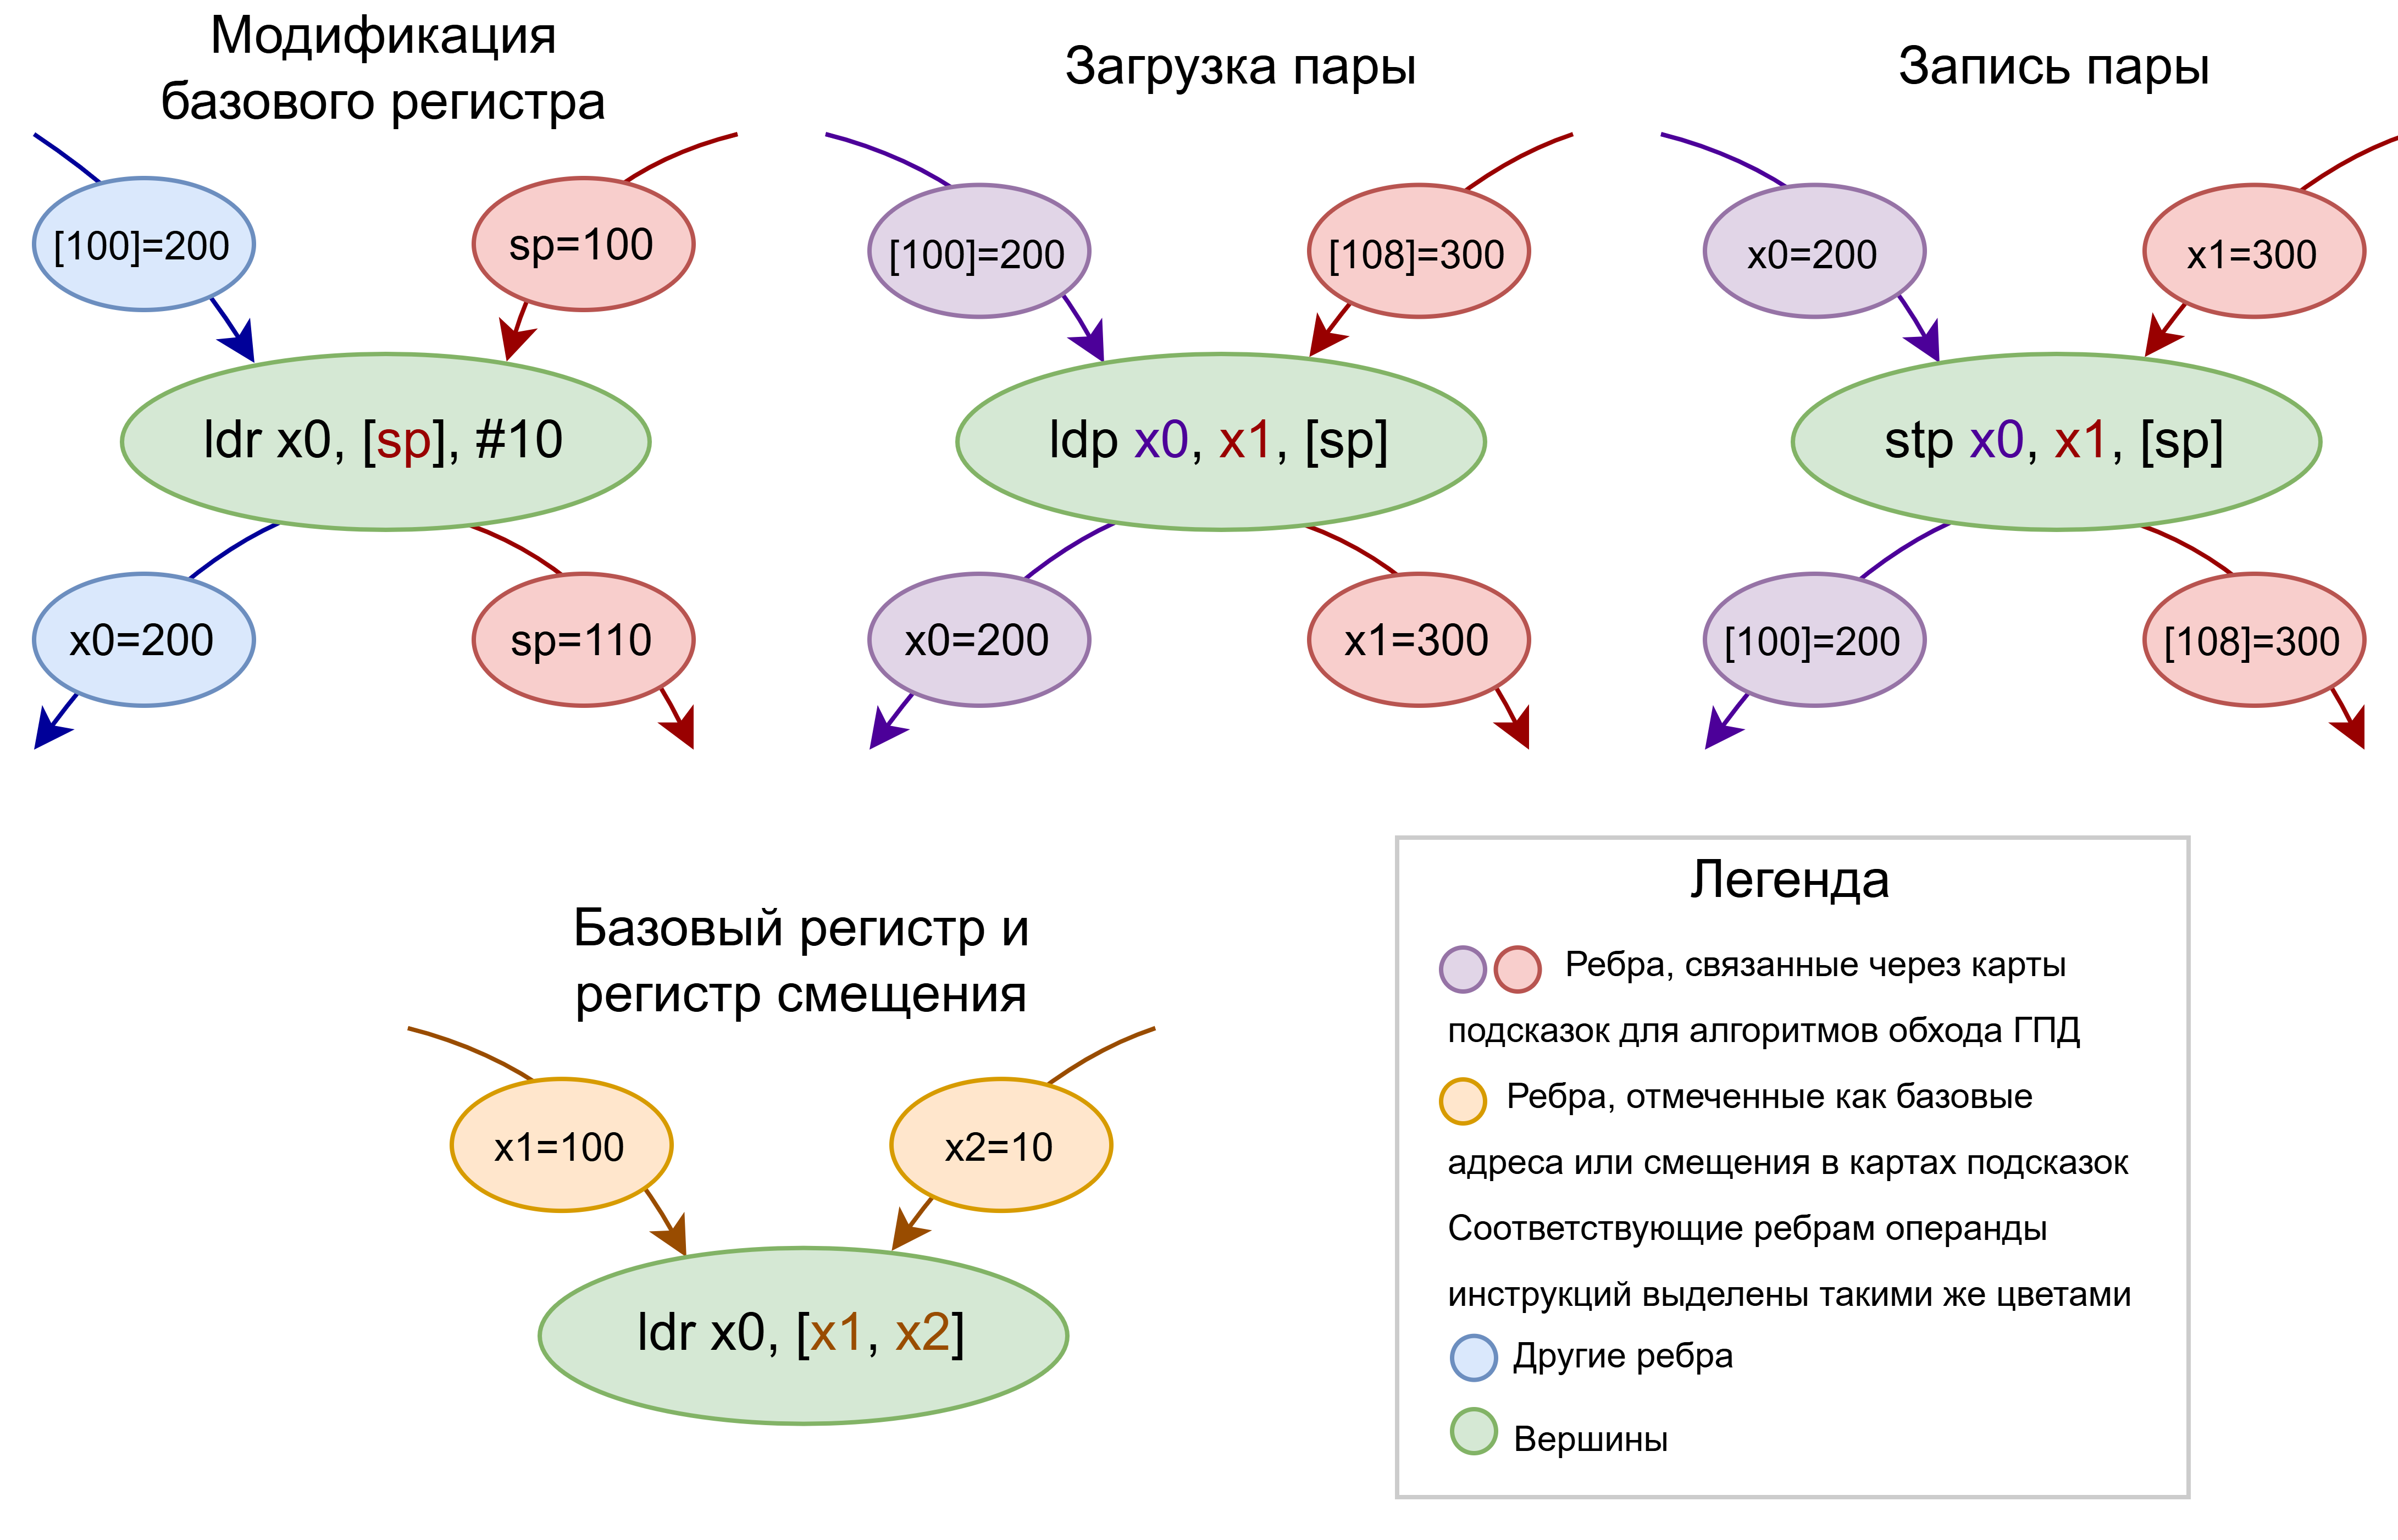
\includegraphics[width=0.8\linewidth]{pics/heuristics_hints.drawio.png}
    \caption{Примеры фрагментов ГПД и сформированных для них подсказок.}
    \label{fig:heuristics_hints}
\end{figure}

На рис. \ref{fig:dfg_uml} представлена UML диаграмма \cite{omg_uml_specification,selic_uml_overview} модуля, отвечающего за сбор и анализ графа потока данных (модуль ГПД).

\begin{figure}[h!]
    \centering
    \includegraphics[width=0.9\linewidth]{pics/dfg_uml.drawio.png}
    \caption{UML диаграмма модуля ГПД.}
    \label{fig:dfg_uml}
\end{figure}
\FloatBarrier

\subsection{Генерация модификаций трассы}

Для генерации трасс с консистентными потоками управления и данных, необходимо поддержать модификации для следующих данных трассы (см. раздел \ref{sec:execution_traces}):

\begin{itemize}
    \item Начальное регистровое состояние

    Начально регистровое состояние может содержать адреса, которые необходимо заменить в соответствии с картой перемещений.

    \item Обращения к памяти

    Обращения к памяти должны происходить по измененным адресам. Также, данные этих обращений могут сами по себе быть адресами.

    \item Значения регистров общего назначения

    Регистровые значения, используемые в качестве адресов, должны быть заменены.
\end{itemize}

Для упрощения задачи запретим добавлять записи типа "обращение в память" и модифицировать размеры и типы обращений для существующих записей: поток данных выходной трассы должен быть похож на исходный, но с замененными адресами. Таким образом, будут использованы четыре вида модификаций для записей трассы (три из которых генерируются на рассматриваемой стадии обработки):

\begin{itemize}
    \item Модификации начального регистрового состояния

    \item Модификации чтений из памяти

    \begin{itemize}
        \item Данные могут быть заменены, если из памяти читается значение, используемое в дальнейшем в качестве адреса.
        \item Адрес чтения должен быть получен из исходного с помощью карты перемещений.
        \item Новые записи не добавляются.
    \end{itemize}

    \item Модификации записей в память

    \begin{itemize}
        \item Данные получаются из симуляции: в память может записываться перемещенный адрес (возможно, преобразованный) или старые данные.
        \item Адрес записи должен быть получен из исходного с помощью карты перемещений.
        \item Новые записи не добавляются.
        \item Не генерируются на рассматриваемой стадии обработки: преобразования тривиальные и осуществляются при записи выходной трассы.
    \end{itemize}

    \item Модификации записей в регистры общего назначения

    \begin{itemize}
        \item Регистровые значения для существующих записей могут быть изменены.
        \item Могут быть добавлены новые записи, исправляющие потоки управления и данных.
    \end{itemize}
\end{itemize}

Генерация модификаций происходит в два этапа:

\begin{enumerate}
    \item Поиск адресов и смещений на ГПД

    На этом этапе производится поиск ребер, значения которых (возможно, после некоторых преобразований) используются в качестве адресов. Для найденных ребер генерируются первичные модификации трассы.

    \item Симуляционный проход по модифицированной трассе

    На этом этапе детектируются расхождения потока управления и потока данных симулятора с ожидаемым поведением на модифицированной трассе. При детектировании расхождений генерируются вторичные модификации трассы, исправляющие ошибки.
\end{enumerate}

Предложенный алгоритм по построению поддерживает любые паттерны адресации в трассе, но может генерировать трассы с большим количеством компенсаций. Подробнее свойства предложенного алгоритма будут рассмотрены в дальнейшем.

\subsubsection{Поиск адресов и смещений}

Введем два маркера для ребер ГПД: красный маркер отмечает ребра, обработанные в ходе обратного обхода ГПД; зеленый маркер отмечает ребра, попавшие в очередь прямого обхода ГПД. В данную очередь будем помещать только ребра, еще не покрашенные зеленым маркером.

Будем называть два ребра близкими по значению если абсолютная разность их значений меньше некоторого порогового значения, являющегося гиперпараметром решения (обозначим как ADDR\_SIMILARITY\_THRESHOLD). Также будем называть ребро $e \in F \subseteq E$ ближайшим по значению к ребру $g$ среди ребер $F$, если $e$ и $g$ близки по значению и пара $(e, g)$ обладает минимальной абсолютной разностью значений среди всех пар $F \times \{g\}$.

Сначала с ГПД собираются ребра, значения которых используются целевыми инструкциями в качестве адресов или считаются адресами по другим косвенным признакам (\glsdisp{addr_edge}{адресные ребра}). К таким значениям относятся: базовые адреса обращений в память; адреса переходов потока управления; адреса, используемые для операций с кешами; значения, которые сравниваются с адресами или вычитаются из них; и т.п.

Для каждого адресного ребра, строится обратный путь на ГПД, начинающийся с этого ребра. Построение выполняется последовательно. На каждом шаге для текущего конечного ребра пути (обозначим это ребро как $e$) выбирается следующее ребро из множества рёбер, входящих в начальную вершину $e$. Построение пути осуществляется до выполнения одного из условий останова: достижения псевдо-инструкции; ошибки поиска следующего ребра; достижения ребра, окрашенного красным маркером; и т.п. Конечное ребро построенного пути будем называть \glsdisp{src_addr_edge}{исходным адресным ребром}. Для таких ребер, а также ребер пути с локациями в памяти, генерируются первичные модификации трассы, что позволяет заменить больш\'{у}ю часть используемых адресов (так как изменения будут распространяться по потоку данных) путем малого количества модификаций трассы. Все ребра построенного пути красятся красным маркером, а исходные адресные ребра также помещаются в очередь прямого обхода ГПД (если они еще не окрашены зеленым маркером). Блок схема алгоритма построения обратных путей на ГПД представлена на рис. \ref{fig:addr_source_search}.

\begin{figure}[h!]
    \centering
    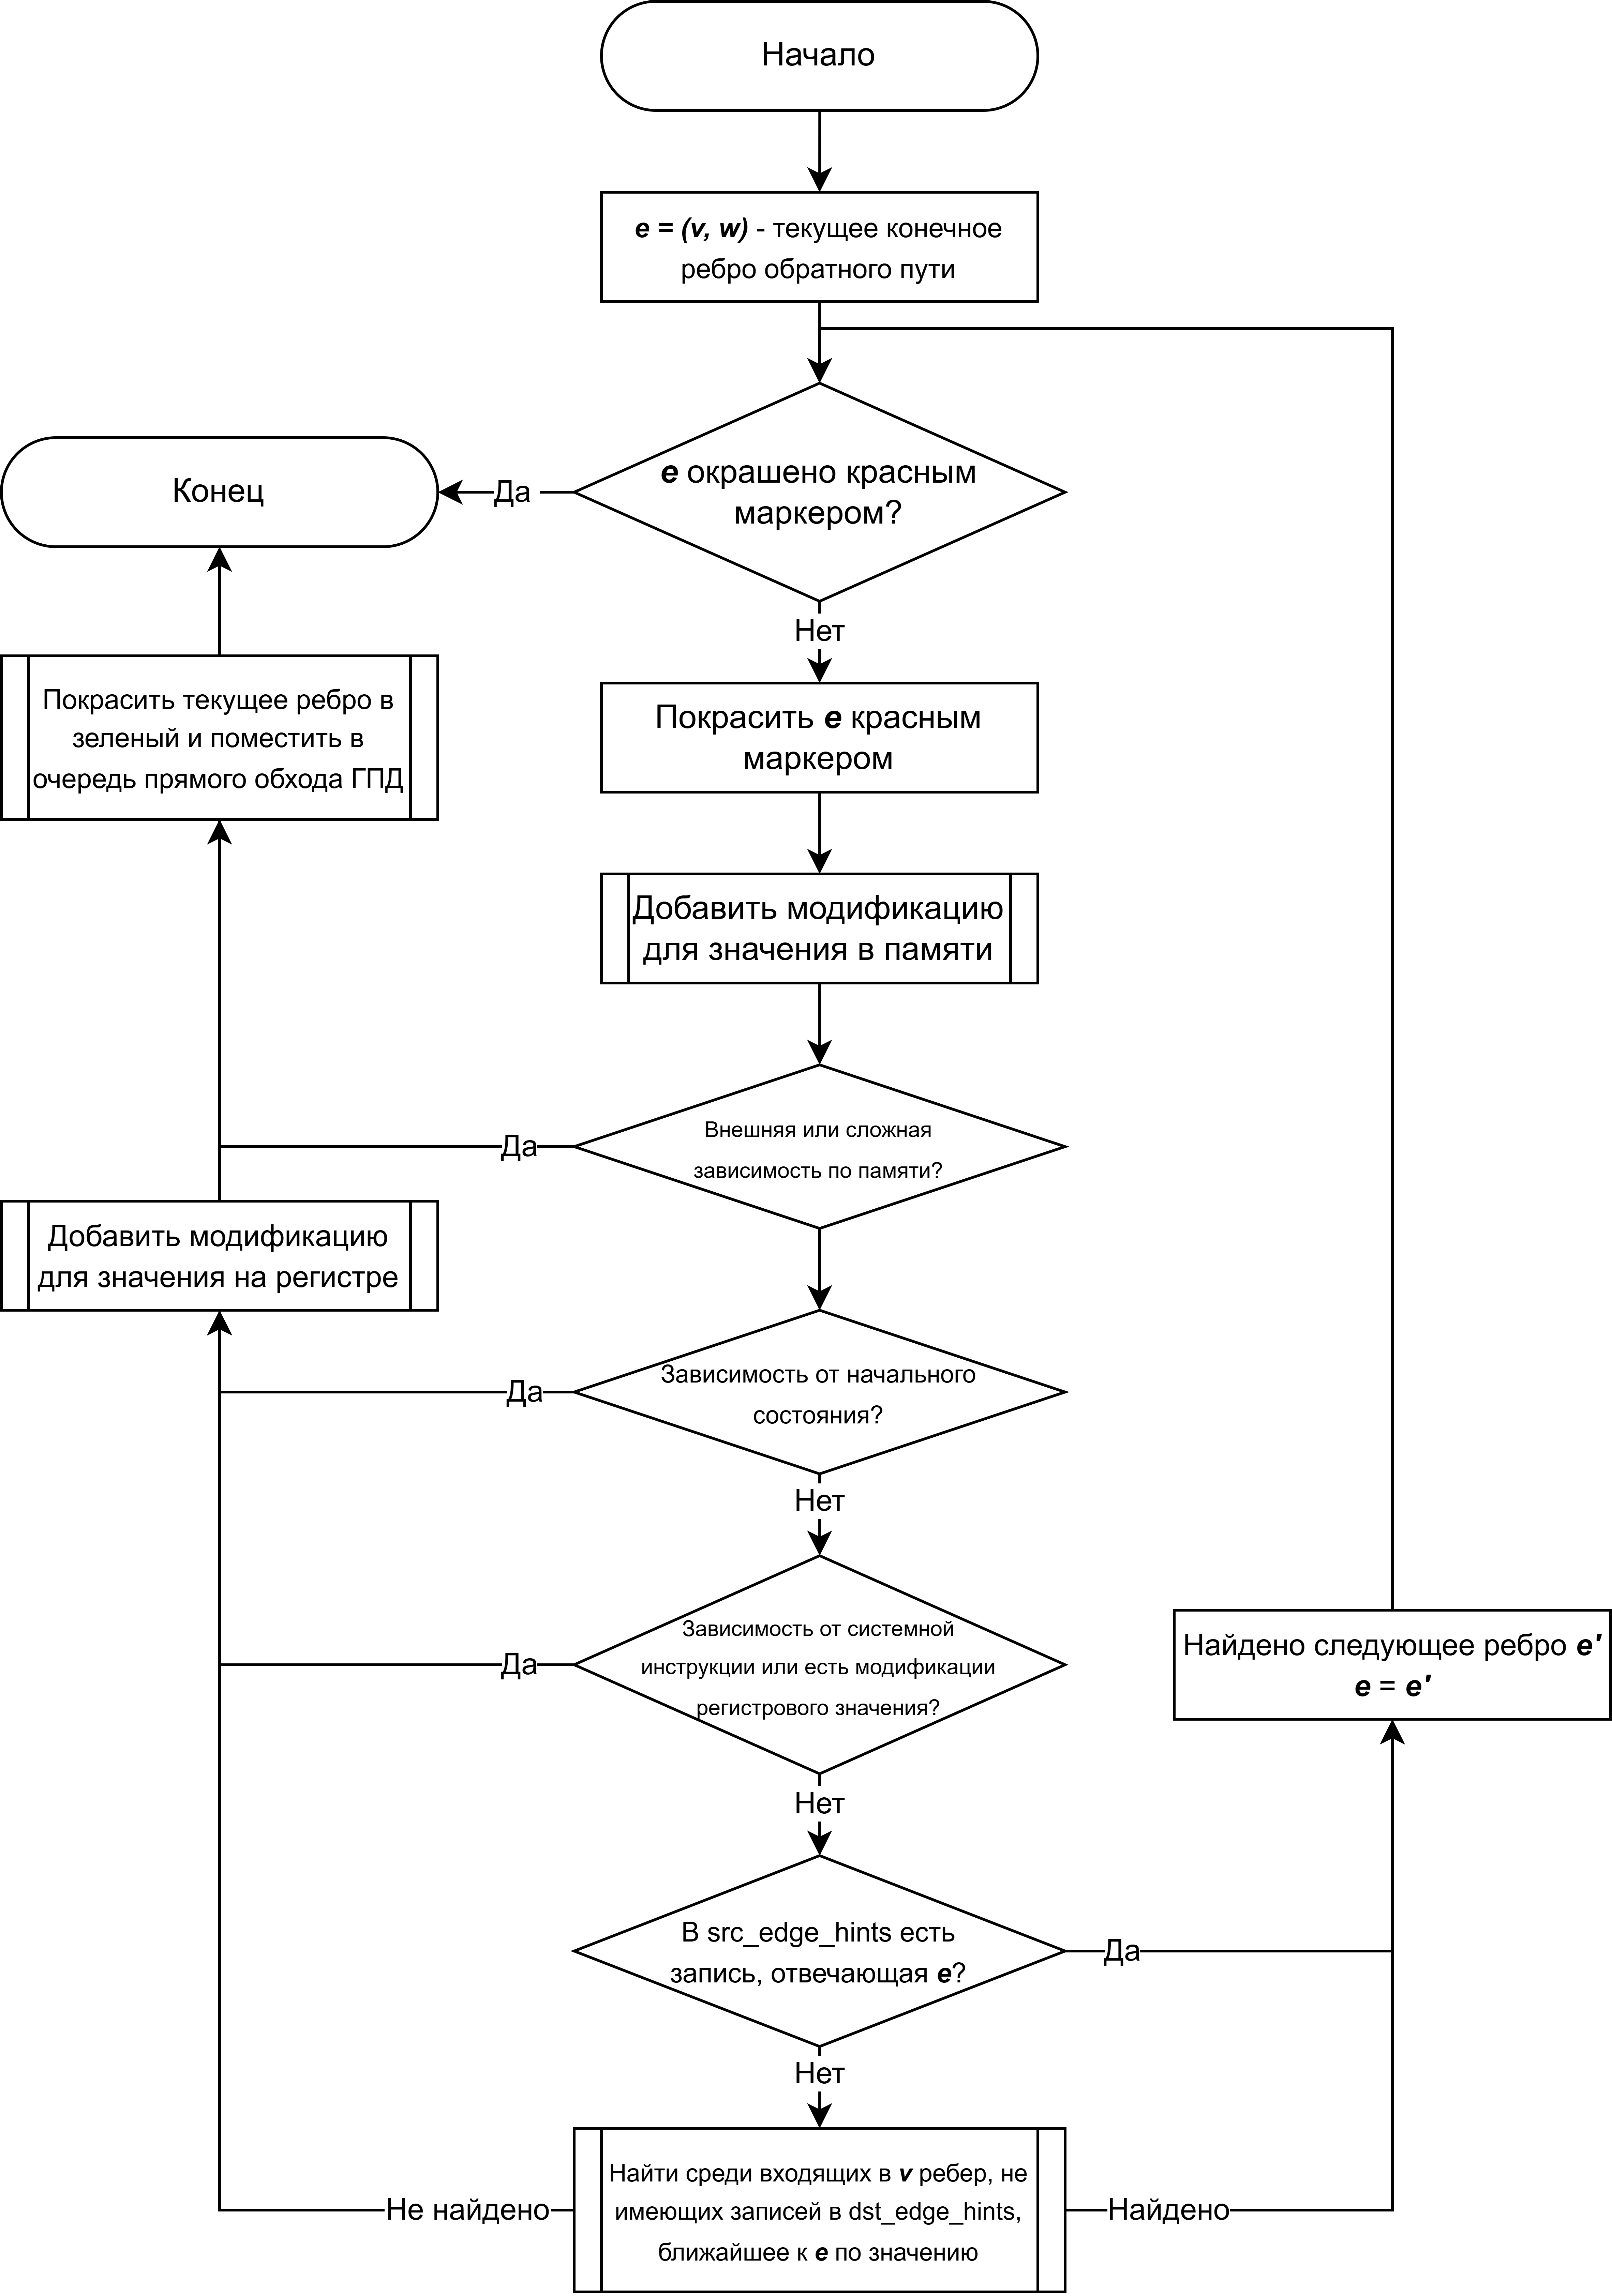
\includegraphics[width=0.8\linewidth]{pics/addr_source_search.drawio.png}
    \caption{Блок схема алгоритма построения обратных путей на ГПД.}
    \label{fig:addr_source_search}
\end{figure}

Затем производится обработка ребер в очереди прямого обхода ГПД. Для каждого ребра $e$ строится обратный путь (если он еще не был построен) и осуществляется поиск ребер для дальнейшего обхода. Найденные ребра добавляются в очередь прямого обхода:

\begin{itemize}
    \item Ребра с такой же начальной вершиной и локацией

    \item Ребра, значения которых сравниваются со значением $e$

    Если $e$ входит в вершину $v$, являющуюся инструкцией сравнения, то все входные ребра $v$ добавляются в очередь.

    \item Ребра, значения которых участвуют в вычитании со значением $e$

    Сценарий аналогичен предыдущему, но значения добавляемых ребер должны быть больше некоторого порогового значения, являющегося гиперпараметром решения (обозначим как ADDR\_MIN\_VALUE).

    \item Ребра, соответствующие $e$ в dst\_edge\_hints.

    \item Ребра, выходящие из $v$, близкие по значению к $e$

    Данные ребра добавляются только если для $e$ нет записей в dst\_edge\_hints.
\end{itemize}

\FloatBarrier

Прямой обход ГПД позволяет найти дополнительные адресные ребра для построения обратных путей на графе и генерации первичных модификаций. Этот обход нужен, так как часть значений в трассе может не использоваться в качестве адресов напрямую, но может сравниваться с адресами, использоваться для подсчета хеш сумм адресов, и т. п. Часть таких значений будет найдена при данном обходе, что позволит в дальнейшем сделать меньше вторичных модификаций (которые всегда снижают репрезентативность трассы).

\subsubsection{Симуляционный проход по модифицированной трассе} \label{sec:patched_trace_sim}

На данной стадии производится проход по трассе, аналогичный изображенному на рис. \ref{fig:trace_simulation}. Но записи трассы преобразуются в соответствии со сгенерированными модификациями. Также до и после каждого симуляционного шага потоки управления и данных симулятора проверяются на расхождения с ожидаемым поведением. При детектировании расхождения, состояние симулятора исправляется и генерируются вторичные модификации трассы, соответствующие исправлению. В случае расхождения после симуляционного шага, состояние симулятора восстанавливается и шаг делается повторно (с примененными исправлениями). Описанный подход позволяет генерировать трассы с консистентными потоками управления и данных. Блок схема алгоритма представлена на рис. \ref{fig:patched_trace_sim}.

\begin{figure}[h!]
    \centering
    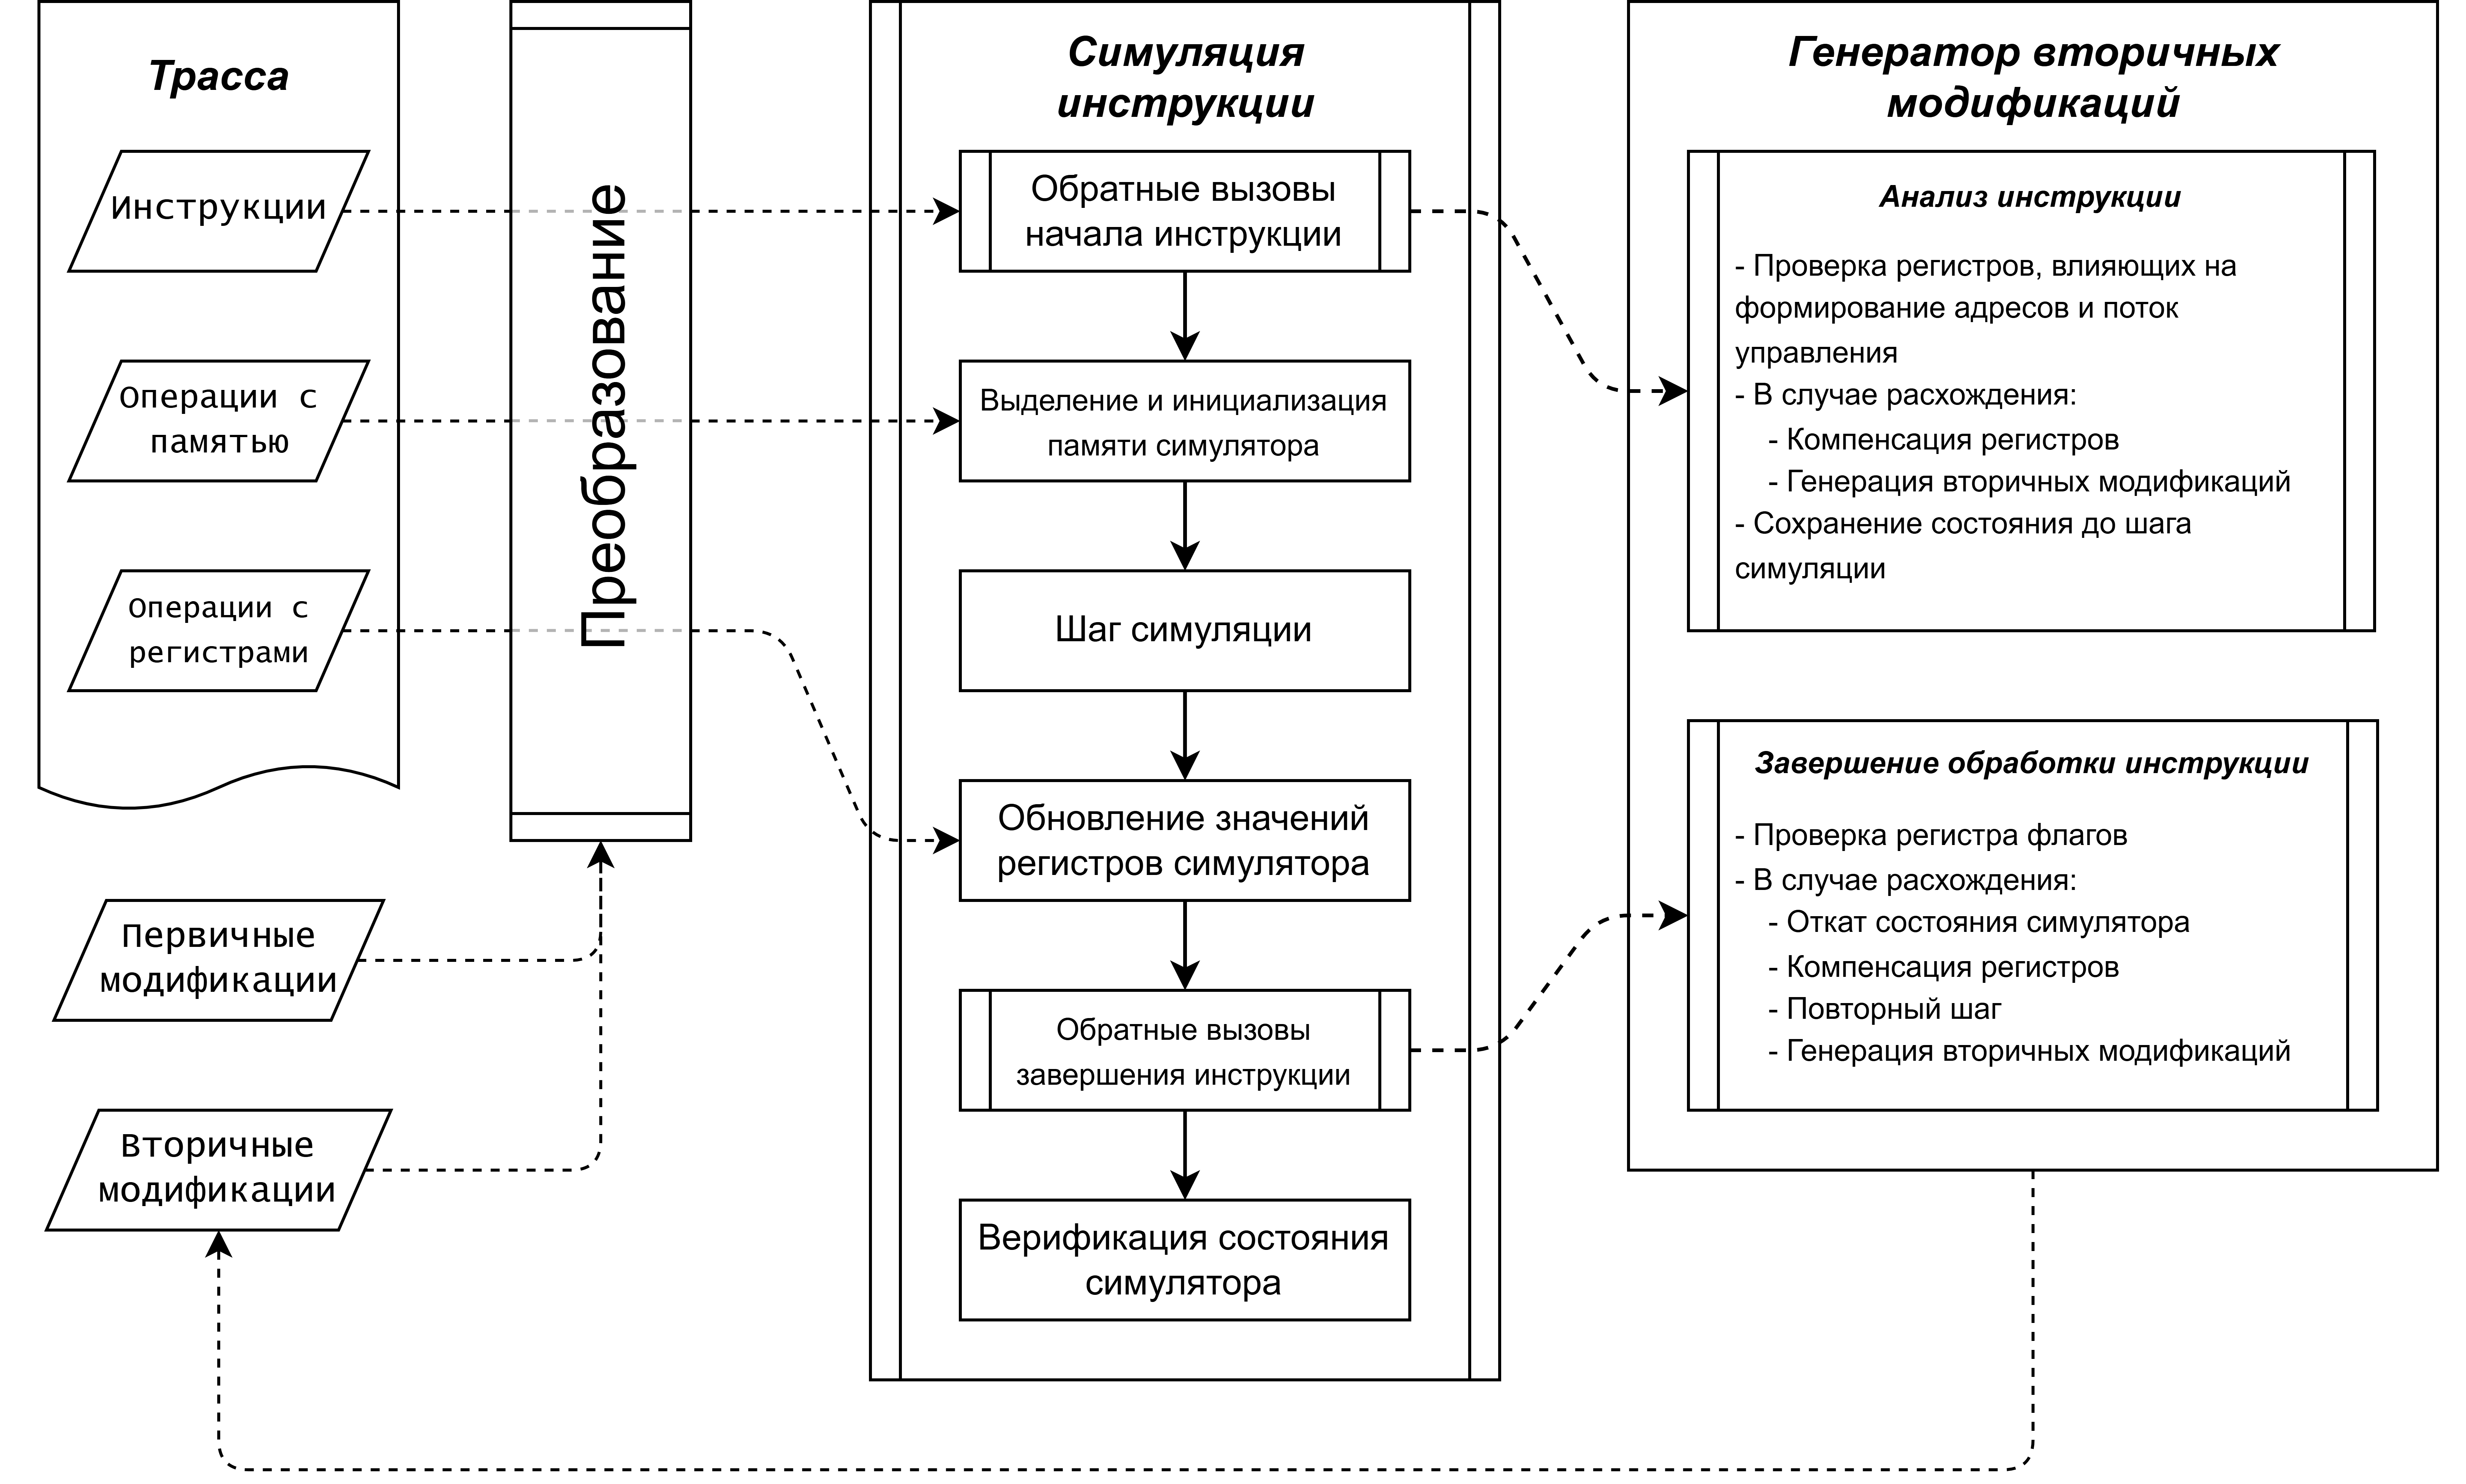
\includegraphics[width=\linewidth]{pics/patched_trace_sim.drawio.png}
    \caption{Блок схема симуляционного прохода по модифицированной трассе.}
    \label{fig:patched_trace_sim}
\end{figure}

\FloatBarrier

\subsection{Запись модифицированной трассы} \label{sec:trace_write}

На данной стадии обработки происходит проход по исходной трассе, в ходе которого оригинальные записи преобразуются с помощью подготовленных модификаций (первичных и вторичных) и записываются в выходную трассу. Так же во время обработки происходит симуляция по модифицированной трассе, аналогичная подходу описанному в разделе \ref{sec:patched_trace_sim}. Симуляция используется для верификации записываемой трассы и получения данных для некоторых записей.

\subsection{Симуляция по трассе}

Рассмотрим подробнее симуляцию по трассе, ранее упомянутую в разделах \ref{sec:execution_traces}, \ref{sec:dfg_collection}, \ref{sec:patched_trace_sim} и \ref{sec:trace_write}. В процессе симуляции данные из трассы пробрасываются в состояние симулятора; таким образом воспроизводится записанное в трассе исполнение и собираются необходимые данные, отсутствующие в трассе (например, значения регистров в определенных точках). Также обычно проверяется консистентность потоков управления и данных.

Для ряда рассмотренных задач применяется симуляция по модифицированной трассе. Заметим, что модифицированная трасса при этом еще не записана в выходной файл, а конструируется на лету из записей исходной трассы и подготовленных модификаций. Функционал обычной симуляции по трассе получается повторно использовать с помощью наследования и переопределения виртуальных функций. Переопределенные методы-обработчики подменяют исходные записи трассы (и/или добавляют новые), а после вызывают методы базового класса на полученных данных. Пример переопределенного метода для обработки модифицированной трассы приведен в листинге \ref{lst:sim_override}.

\begin{listing}[htbp]
    \inputminted{c++}{listings/sim_override.cpp}
    \caption{Переопределение метода-обработчика записей доступа в память}
    \label{lst:sim_override}
\end{listing}

Также класс симулятора по трассе поддерживает добавление обратных вызовов (callback), что позволяет повторно использовать его для различных симуляционных задач решения. На рис. \ref{fig:sim_uml} представлена UML-диаграмма классов симуляционного модуля.

\begin{figure}[h!]
    \centering
    \includegraphics[width=\linewidth]{pics/sim_uml.drawio.png}
    \caption{UML-диаграмма классов симуляционного модуля.}
    \label{fig:sim_uml}
\end{figure}

\FloatBarrier

\subsection{Тестирование}

Для тестирования \glsdisp{sw}{программного обеспечения} (ПО) часто применяются следующие подходы:

\begin{itemize}
    \item \gls{unit-testing} -- проверяется корректность работы отдельных функций или методов изолированно от других компонентов \cite{googletest_documentation,catch2_documentation,boost_test_documentation}.
    \item \gls{module-testing} -- проверяется работа отдельных модулей. Тестируются корректность взаимодействий внутри модуля и его интерфейсов.
    \item \gls{end-to-end-testing} -- решение тестируется полностью на целевых сценариях и данных.
\end{itemize}

Для юнит- и модульного тестирования решения используются фреймворк GoogleTest \cite{googletest_documentation} и тестовая инфраструктура используемой системы сборки CMake \cite{cmake_ctest_documentation,hoffman_martin_cmake}. Также возможно добавление сквозных тестов с использованием реальных или синтетических трасс и инфраструктуры проекта.

Дизайн ключевых компонентов решения позволяет применять юнит- и модульное тестирование, возможно, после нескольких незначительных изменений. Основной задачей для поддержки подобного тестирования является отделение компонентов решения от библиотеки для чтения трасс. Это позволит осуществлять частичную обработку тестовых данных без наличия реальной трассы. Примером подобного отделения является публичный интерфейс модуля ГПД (см. рис. \ref{fig:dfg_uml}): класс \textit{DfgCollector} принимает данные, не привязанные явно к библиотеке для чтения трасс (хотя формат данных сильно похож на формат записей трассы). Это позволяет собирать ГПД и вспомогательные данные на тестовых сценариях, а затем проверять консистентность, инварианты и выполнение тестовых условий. Для упрощения описания тестовых сценариев была реализована вспомогательная инфраструктура, в упрощенном виде представленная в листингах \ref{lst:testing_dfg_builder} и \ref{lst:testing_dfg_collector}. Пример юнит-теста, использующего описанную инфраструктуру, представлен в листинге \ref{lst:testing_dfg_collector_example}.

С помощью описанной тестовой инфраструктуры было добавлено 7 юнит-тестов, покрывающих базовый функционал для работы с ГПД и ряд краевых случаев. Примененный подход показал свою эффективность: тестовые сценарии описываются легко и могут быть повторно использованы несколькими тестами для проверки различных компонентов. Полное тестирование модуля ГПД и других модулей может быть осуществлено в рамках дальнейшего развития решения.

\begin{listing}[htbp]
    \inputminted{c++}{listings/testing_dfg_builder.cpp}
    \caption{Класс для генерации тестовых ГПД.}
    \label{lst:testing_dfg_builder}
\end{listing}

\begin{listing}[htbp]
    \inputminted{c++}{listings/testing_dfg_collector.cpp}
    \caption{Класс-фикстура для юнит-тестирования класса DfgCollector.}
    \label{lst:testing_dfg_collector}
\end{listing}

\begin{listing}[htbp]
    \inputminted{c++}{listings/testing_dfg_collector_example.cpp}
    \caption{Пример юнит-теста для класса DfgCollector.}
    \label{lst:testing_dfg_collector_example}
\end{listing}

\FloatBarrier

\subsection{Оценка решения}

В данном разделе будет произведена оценка решения.

\subsubsection{Пространственная и временная сложность}

Рассмотрим алгоритмическую сложность \cite{clrs_algorithms} решения. Размеры трассы и количество итераций при проходе по ней пропорциональны количеству инструкций в трассе $N = |V|$.

Рассмотри временную и пространственную сложность стадий обработки трассы:

\begin{itemize}
    \item Генерация карты перемещений

    Временная сложность - $O(N)$ (полный проход по трассе).
    Пространственная сложность - $O(N)$ (агрегация данных с записей трассы).

    \item Сбор ГПД

    Временная сложность - $O(N)$ (полный проход по трассе).
    Пространственная сложность - $O(N + K)$. Где $K = |E|$ - количество ребер ГПД.

    \item Генерация модификаций трассы

    На данной стадии производится два обхода ГПД: построение обратных путей и прямой обход. При этом ни одно ребро не обходится дважды, так как обработанные ребра отмечаются маркерами. Временная сложность обходов графа - $O(N + K)$. Также в конце производится симуляционный проход по модифицированной трассе, временная сложность - $O(N)$.

    Результирующая временная сложность - $O(N + K)$

    На данной стадии генерируются модификации трассы, количество которых пропорционально количеству инструкций и количеству ребер ГПД. Пространственная сложность - $O(N + K)$.

    \item Модификация трассы

    Временная сложность - $O(N)$ (полный проход по трассе).
    Пространственная сложность - $O(1)$.
\end{itemize}

Заметим, что выполняется асимптотическая оценка: $K = O(N)$. Таким образом, пространственная и временная сложность обработки трассы $O(N + K) = O(N)$.

\subsubsection{Оценка репрезентативности трасс}

Для оценки репрезентативности выходных трасс будет использоваться статистика произведенных модификаций. Рассмотрим различные модификации трассы и их влияние на репрезентативность:

\begin{itemize}
    \item Замена адреса для операции с памятью - не влияет на репрезентативность, так как не требует компенсации при дальнейшей обработке выходной трассы.

    \item Замена значения для записи в память - не требует компенсации (поток данных консистентен).

    \item Замена значения для чтения из памяти - может влиять на репрезентативность в некоторых сценариях. При чтении значения, не соответствующего текущему образу памяти рассматриваемого потока, может потребоваться компенсация, аналогичная компенсации для внешней модификации памяти. Заметим, что если в оригинальной трассе уже присутствовала внешняя модификация памяти, модификация не повлияет на репрезентативность.

    \item Замена значения регистра в начальном состоянии - не требует дополнительной компенсации.

    \item Замена значения для записи в регистр общего назначения - не требует дополнительной компенсации.

    \item Добавление записи в регистр общего назначения - требует компенсации, будет снижать репрезентативность.
\end{itemize}

Таким образом, для оценки влияния на репрезентативность трасс будем использовать кумулятивную метрику $N_{comp}$ - количество модификаций, приводящих к появлению дополнительных компенсаций при обработке трассы. Обозначим также $P_{comp} = \frac{N_{comp}}{|V|}$ - количество компенсируемых модификаций на инструкцию трассы.

\subsubsection{Профилировка решения по памяти} \label{sec:memory_profiling}

Для получения грубой оценки потребления памяти различными компонентами использовалась утилита heaptrack \cite{heaptrack_documentation}, позволяющая отследить объемы выделений памяти различными участками кода. Данные heaptrack для набора тестовых трасс показывают, что в коде библиотеки Boost Graph выделяется больше 90 процентов используемой памяти.

\subsubsection{Тестовые запуски на целевых трассах} \label{sec:real_trace_tests}

В данном разделе будут представлены результаты тестовых запусков на целевых трассах заказчика (таблица \ref{tab:real_traces_tests}). Рассматриваются следующие метрики:

\begin{itemize}
    \item $N$ - количество инструкций в трассе.
    \item $N_{comp}$ - количество компенсируемых модификаций.
    \item $P_{comp} = \frac{N_{comp}}{N}$ - количество компенсируемых модификаций на инструкцию трассы.
    \item $RSS_{max}$ - максимальный объем резидентной памяти (resident set size) \cite{gnu_time_memory_resources,linux_proc_filesystem}, занятый при модификации трассы.
    \item $P_{RSS} = \frac{RSS_{max}}{N}$ - объем резидентной памяти на инструкцию трассы.
    \item $T$ - время обработки трассы.
    \item $V = \frac{N}{T}$ - средняя скорость обработки (инструкций в секунду).
\end{itemize}

\begin{table}[htbp]
\centering \small

\caption{Результаты тестовых запусков на целевых трассах заказчика}
\label{tab:real_traces_tests}

\begin{tabular}{|p{3.6cm}|l|l|l|l|l|l|l|} \hline
    \textbf{Трасса}         & $\mathbf{N}$ & $\mathbf{N_{comp}}$ & $\mathbf{P_{comp}}$ & $\mathbf{RSS_{max}},$ & $\mathbf{P_{RSS}},$         & $\mathbf{T},\,\texttt{С}$ & $V,\,\frac{1}{\texttt{С}}$ \\
    \textbf{(тип нагрузки)} &              &                     &                     & $\texttt{Гб}$         & $\frac{\texttt{Гб}}{10^6}$  &                           &                               \\ \hline

    LogicTrace1 \linebreak (вычислительная) & $1.7 \cdot 10^{7}$ & $3.7 \cdot 10^{5}$ & $2.1 \cdot 10^{-2}$ & $7.65$  & $0.44$ & $162.5$ & $1.07 \cdot 10^{5}$ \\ \hline

    LogicTrace2 \linebreak (вычислительная) & $1.6 \cdot 10^{7}$ & $4.0 \cdot 10^{5}$ & $2.5 \cdot 10^{-2}$ & $6.91$  & $0.44$ & $149.3$ & $1.06 \cdot 10^{5}$ \\ \hline

    LogicTrace3 \linebreak (вычислительная) & $4.1 \cdot 10^{7}$ & $9.5 \cdot 10^{4}$ & $2.3 \cdot 10^{-3}$ & $16.71$ & $0.41$ & $408.7$ & $1.00 \cdot 10^{5}$ \\ \hline

    LogicTrace4 \linebreak (вычислительная) & $1.6 \cdot 10^{7}$ & $7.4 \cdot 10^{3}$ & $4.5 \cdot 10^{-4}$ & $6.91$  & $0.43$ & $160.0$ & $1.05 \cdot 10^{5}$ \\ \hline

    LogicTrace5 \linebreak (вычислительная) & $3.4 \cdot 10^{7}$ & $1.3 \cdot 10^{3}$ & $4.1 \cdot 10^{-5}$ & $13.38$ & $0.40$ & $321.3$ & $1.04 \cdot 10^{5}$ \\ \hline

    GfxTrace1 \linebreak (графика)          & $1.0 \cdot 10^{7}$ & $7.0 \cdot 10^{3}$ & $6.7 \cdot 10^{-4}$ & $4.47$  & $0.43$ & $99.3$  & $1.05 \cdot 10^{5}$ \\ \hline
\end{tabular}

\end{table}

Обозначим: $M$ - количество тестовых трасс. Рассчитаем средние значения для $\mathbf{P_{comp}}$, $\mathbf{P_{RSS}}$ и $V$.

Для $\mathbf{P_{comp}}$ приведено среднее арифметическое - доля компенсированных инструкций характеризует качество выходной трассы, подобное усреднение позволит оценить долю компенсаций в случайно выбранной трассе. При этом не учитываются размеры тестовых трасс, так как на долю компенсаций в первую очередь влияют особенности потоков данных и управления. Также для $\mathbf{P_{comp}}$ приведен 50-й процентиль (медиана), так как на ряде тестовых трасс доля компенсаций существенно выше, что может говорить о наличии большого количества еще не поддержанных краевых случаев. \\

$\displaystyle \overline{P_{comp}} = \frac{1}{M} \sum_{i=1}^{M} P_{comp_i} = 8.3 \cdot 10^{-3} $ \\

$ \displaystyle P_{50}\left(P_{comp}\right) = 6.7 \cdot 10^{-4} $ \\

$\mathbf{P_{RSS}}$ также усреднено с помощью среднего арифметического - потребление памяти линейно от количества инструкций (остальные накладные расходы пренебрежимо малы). Значит потребление памяти на одну инструкцию также будет в первую очередь зависеть от свойств потоков управления и данных (например от количества ребер на одну инструкцию), но не от размеров трасс. Подобная оценка позволит оценить максимальное суммарное количество инструкций в наборе трасс, который можно обрабатывать одновременно в условиях ограниченной памяти. \\

$\displaystyle \overline{P_{RSS}} = \frac{1}{M} \sum_{i=1}^{M} P_{RSS_i} = 0,42 \frac{\texttt{Гб}}{10^6} $ \\

Для $V$ приведено взвешенное гармоническое среднее, являющееся средней скоростью обработки всего массива тестовых трасс. \\

$\displaystyle \overline{V} = \frac{\displaystyle \sum_{i=1}^{M} N_i}{\displaystyle \sum_{i=1}^{M} T_i} = 103334 \frac{1}{\texttt{С}}$ \\

\subsection{Возможные направления дальнейшего развития решения}

\subsubsection{Поддержка краевых случаев}

Компенсация ряда часто встречающихся краевых случаев может быть оптимизирована с помощью дополнительного анализа или добавления специализированных записей, компенсация которых может быть упрощена. Примеры возможных оптимизаций:

\paragraph {32-битные адресные значения}

Некоторые среды выполнения на 64-битных платформах используют компактные 32-битные представления ссылок для снижения потребления памяти: подобные представления используются в Android Runtime, HotSpot JVM и V8 \cite{android_art_object_reference,openjdk_compressed_oops,v8_pointer_compression}. Свободные биты указателей могут использоваться для хранения метаданных \cite{android_tagged_pointers,v8_pointer_compression}. При модификации такого компактного адреса новое значение может не помещаться в исходное представление. В подобных случаях появляются типовые компенсации: выставление нескольких старших бит адреса (часто одинаковых от обращения к обращению). Для таких случаев можно добавлять в трассу специализированные записи, которые позволят компенсировать только эти старшие биты, что может существенно улучшить репрезентативность для ряда сценариев. Подобная оптимизация требует поддержки в обработчиках трасс.

\paragraph{Хеширование адресов}

Для оптимизации компенсаций хешей адресов можно детектировать хеш функции по символьной информации (в случае полноценного вызова) и/или с помощью специализированного алгоритма, детектирующего хеширование на ГПД (при отсутствии символьной информации или инлайнинге) - с помощью методов сопоставления сигнатур графов \cite{binary_code_similarity_survey,graph_matching_survey}, символьного исполнения \cite{king_symbolic_execution} и SAT решателей \cite{handbook_of_satisfiability}.

\subsubsection{Оптимизация по памяти}

В разделе \ref{sec:real_trace_tests} приведено потребление RAM памяти во время тестовых запусков на реальных трассах исполнения заказчика (таблица \ref{tab:real_traces_tests}, также приведено усредненное значение). Подобное потребление не позволяет обрабатывать трассы с количеством инструкций порядка $1\cdot10^{9}$ и более при доступном объеме RAM, характерном для инфраструктуры заказчика. Также высокое потребление памяти существенно ограничивает возможности для параллельной обработки наборов трасс. Также в разделе \ref{sec:real_trace_tests} было показано, что основную долю потребляемой RAM занимает ГПД.

Для снижения потребления RAM памяти можно использовать специализированные библиотеки для работы с большими графами \cite{graphchi}. Такие решения хранят графы на диске и подкачивают данные в RAM при необходимости. Также могут быть применены менее специализированные библиотеки: библиотека STXXL \cite{stxxl}, предоставляющая реализации для типовых C++ контейнеров, оптимизированных под большие объемы данных; библиотеки LLNL Metall \cite{llnl_metall} и LLNL Umap \cite{llnl_umap}, предоставляющие высокоуровневые интерфейсы для выделения памяти через отображаемые файлы (ОС может выгружать такую память на диск) и контроля над выгрузкой страниц соответственно, что позволяет использовать эти библиотеки для ограничения используемой RAM.

Другим вариантом решения проблемы является отказ от хранения ГПД для всей трассы. Возможна блочная обработка трассы, со сбором ГПД только для обрабатываемого в данный момент блока. Такой подход потребует многократного сбора одних и тех же участков графа для осуществления всех необходимых обходов графа и обходов трассы, использующих данные графа. Подобное многократное восстановление данных может существенно замедлить обработку трасс, в таком случае потребуются дополнительные оптимизации.

\subsubsection{Поддержка векторных регистров}

В данный момент на ГПД добавляются только зависимости по памяти и регистрам общего назначения. При этом векторные регистры также могут использоваться для формирования адресов \cite{arm_sve_introduction}. Добавление информации о значениях векторных регистров на ГПД позволит улучшить качество генерируемых модификаций (можно будет отследить адресные значения на векторных регистрах) и поддержать инструкции, напрямую использующие эти регистры для формирования адресов (например scatter store и gather load инструкции из расширения SVE системы команд ARM64 \cite{arm_sve_introduction}).

\subsubsection{Модификация криптографических подписей адресов}

Представленное решение может быть использовано не только для изменения образа памяти трасс, но и для других задач, требующих поиска адресов в трассе. Одной из подобных задач является замена криптографических подписей адресов.

Криптографические расширения систем команд, такие как расширение PAuth архитектуры ARM64 \cite{arm_pointer_authentication,pacman}, позволяют подписывать используемые адреса и верифицировать их подпись непосредственно перед использованием. Это позволяет защитить систему от ряда кибер атак, основанных на подмене адресов потока управления.

При анализе трасс, содержащих PAuth инструкции, появляется необходимость переподписать адреса из трассы, так как ключ шифрования трассируемой системы может быть неизвестен. Локации подписанных адресов можно искать с помощью описанных в данной работе алгоритмов, после их незначительной корректировки.


\clearpage
 %% Обзор существующих решений
    \section{Заключение}

В рамках работы было представлено решение для модификации трасс исполнения с целью изменения записанных образов памяти трассируемых сценариев для удовлетворения ограничений измененных настроек адресации (отличающихся от настроек трассируемой платформы). Реализованны многопроходные алгоритмы для сбора и анализа графа потока данных, которые позволяют находить локации адресов в трассе и заменять их в соответствии с новыми ограничениями. Решение позволило успешно модифицировать часть целевых трасс заказчика, которые затем прошли верификацию на функциональном симуляторе, проверку репрезентативности и были использованы для анализа производительности разрабатываемых систем с новыми настройками адресации.

Была разработана инфраструктура для описания тестовых сценариев для юнит- и модульных тестов. На основе данной инфраструктуры были написаны базовые тесты для модуля сбора ГПД. Возможно применение данной инфраструктуры для покрытия тестами других модулей.

Рассмотрена базовая методология для оценки репрезентативности (качества) выходных трасс. Представлены метрики, собранные в результате тестовых запусков решения на целевых трассах исполнения заказчика: скорость обработки (инструкций в секунду); потребление памяти (максимальный объем резидентной памяти, расход на одну инструкцию); метрики для оценки репрезентативности.

Приведены возможные направления для дальнейшего развития решения.

\clearpage
 %% Заключение

    \nocite{*}
    \printbibliography
\end{document}
